% --------------------------------------------------------------------------------
% Concepts: Applications
% --------------------------------------------------------------------------------

% ================================================================================
\chapter{Applications}
\hypertarget{Chapter:ConceptsApplications}{}
% ================================================================================

% --------------------------------------------------------------------------------
\section{Introduction}
% --------------------------------------------------------------------------------

Whereas the previous chapters handled the basic modules and a
comparison of their results with psychoacoustic data, this chapter
focuses on some more elaborated applications where these modules
are used in practice. Each of the sections in this chapter
contains:
\begin{itemize}
\item a small introduction in which the purpose of the application is explained
\item a description of the method that is used
\item a summary of how to run the application in practice using
the toolbox and its functions
\item an overview of the obtained results and a discussion thereof
\end{itemize}
The applications are explained from a practical viewpoint, and
each time a link is made between the related concepts and the
practical tools (MATLAB functions) available in the toolbox.\\

The following applications are included:
\begin{itemize}
\item Roughness applications: relationships between timbre, scales and roughness.
\item A rhythmic pattern extraction demonstration for extracting
repetitive rhythm patterns from a sound fragment.
\end{itemize}
Each application can be seen as a demonstration of one (or more)
module(s) that were handled in the first chapter. You can of
course freely experiment with the modules yourself and build some
new applications from the basic functions. If you think that
you've come up with something interesting, we would love to hear
about it!

% --------------------------------------------------------------------------------
% --------------------------------------------------------------------------------
\newpage
\section{Roughness applications}
% --------------------------------------------------------------------------------

% Make target for following functions:
\hypertarget{Concepts:IPEMCalcRoughnessOverSubparts}{}
\hypertarget{Concepts:IPEMGeneratePitchShiftScript}{}

\IPEMTBC (ask Marc for latest version since Koen sent it for that paper)

% --------------------------------------------------------------------------------
\subsection{Introduction}
% --------------------------------------------------------------------------------

% --------------------------------------------------------------------------------
\subsection{Method}
% --------------------------------------------------------------------------------

% --------------------------------------------------------------------------------
\subsection{Application}
% --------------------------------------------------------------------------------

% --------------------------------------------------------------------------------
\subsection{Results and discussion}
% --------------------------------------------------------------------------------

% --------------------------------------------------------------------------------

% --------------------------------------------------------------------------------
% --------------------------------------------------------------------------------
\newpage
\section{Rhythmic pattern extraction}
% --------------------------------------------------------------------------------

% Make target for following functions:
\hypertarget{Concepts:IPEMDemoStartMEC}{}
\hypertarget{Concepts:IPEMDemoMECRhythmExtraction}{}

% --------------------------------------------------------------------------------
\subsection{Introduction}
% --------------------------------------------------------------------------------

In this demonstration, the MEC algorithm from the
\hyperlink{Concepts:RhythmModule}{Rhythm Module (RhM)} is used to
detect and extract rhythmic patterns from a sound fragment.\\
The extracted patterns are then used to synthesize sound using
modulated AM noise, which allows for an auditive comparison
between the original sound and the sound resynthesized from what
the Rhythm Module has extracted.

% --------------------------------------------------------------------------------
\subsection{Method}
% --------------------------------------------------------------------------------

For the extraction of rhythmic patterns, we are interested in
periods ranging from roughly 50 ms to 5 seconds.\\
The signal that will be analyzed is a root-mean-square (RMS)
signal calculated every 10 ms over a frame of 20 ms. We can
calculate the RMS:
\begin{itemize}
\item of the signals in the different channels of the output of
an auditory model (which yields a multi-channel RMS signal)
\item of the sound signal itself (which yields a 1-dimensional RMS signal)
\end{itemize}
This energy signal is then first analyzed using the MEC algorithm
and the most prominent periods occurring in the RMS signal is
detected by finding the minimum in the calculated difference
values. In the first case, this can be done by detecting a minimum
for each channel separately (yields best period for each channel)
or by summing the difference values from all channels first and then
picking the minimum from there (yields a single best period for all channels).\\
Once the best periods are known, the patterns corresponding to
that period can be extracted from the RMS signal.\\
Then, a specific moment in time is chosen, and the extracted
patterns at that moment are used for a resynthesis in order be
able to listen to what the MEC algorithm has found as rhythmic
pattern.\\
For more detailed information on the Rhythm Module itself, see
page \pageref{Concepts:RhythmModule}.\\

% --------------------------------------------------------------------------------
\subsection{Application}
% --------------------------------------------------------------------------------

The contents and the functions for this demo on rhythmic pattern
extraction using MEC can be found in the directory
IPEMToolbox$\backslash$Demos$\backslash$MECPatternExtraction.\\
The main functions are:
\begin{itemize}
\item \hyperlink{FuncRef:IPEMDemoMECRhythmExtraction}{IPEMDemoMECRhythmExtraction}\\
    This demo function starts an interactive session in which you can
    select a sound file, set some basic parameters, analyze the sound using
    MEC and then resynthesize using the analysis results.
\item \hyperlink{FuncRef:IPEMDemoStartMEC}{IPEMDemoStartMEC}\\
    This demo function starts an entire MEC analysis run in one go
    (without interaction). It allows to set more parameters and to save
    the analysis results to a file.
\end{itemize}
Both demo functions are based on the core functions related to the
\hyperlink{Concepts:RhythmModule}{Rhythm Module (RhM)}. You can
have a closer look to the Matlab code of the demo functions to get
to know how these core functions are used, or just check out the
functions in the \hyperlink{Part:ReferenceManual}{Reference
Manual}.


\subsubsection*{Interactive demo}

Figure \ref{Fig:IPEMDemoMECRhythmExtractionChart} shows the
execution flow of IPEMDemoMECRhythmExtraction.

\begin{figure}[!h]
    \centering
    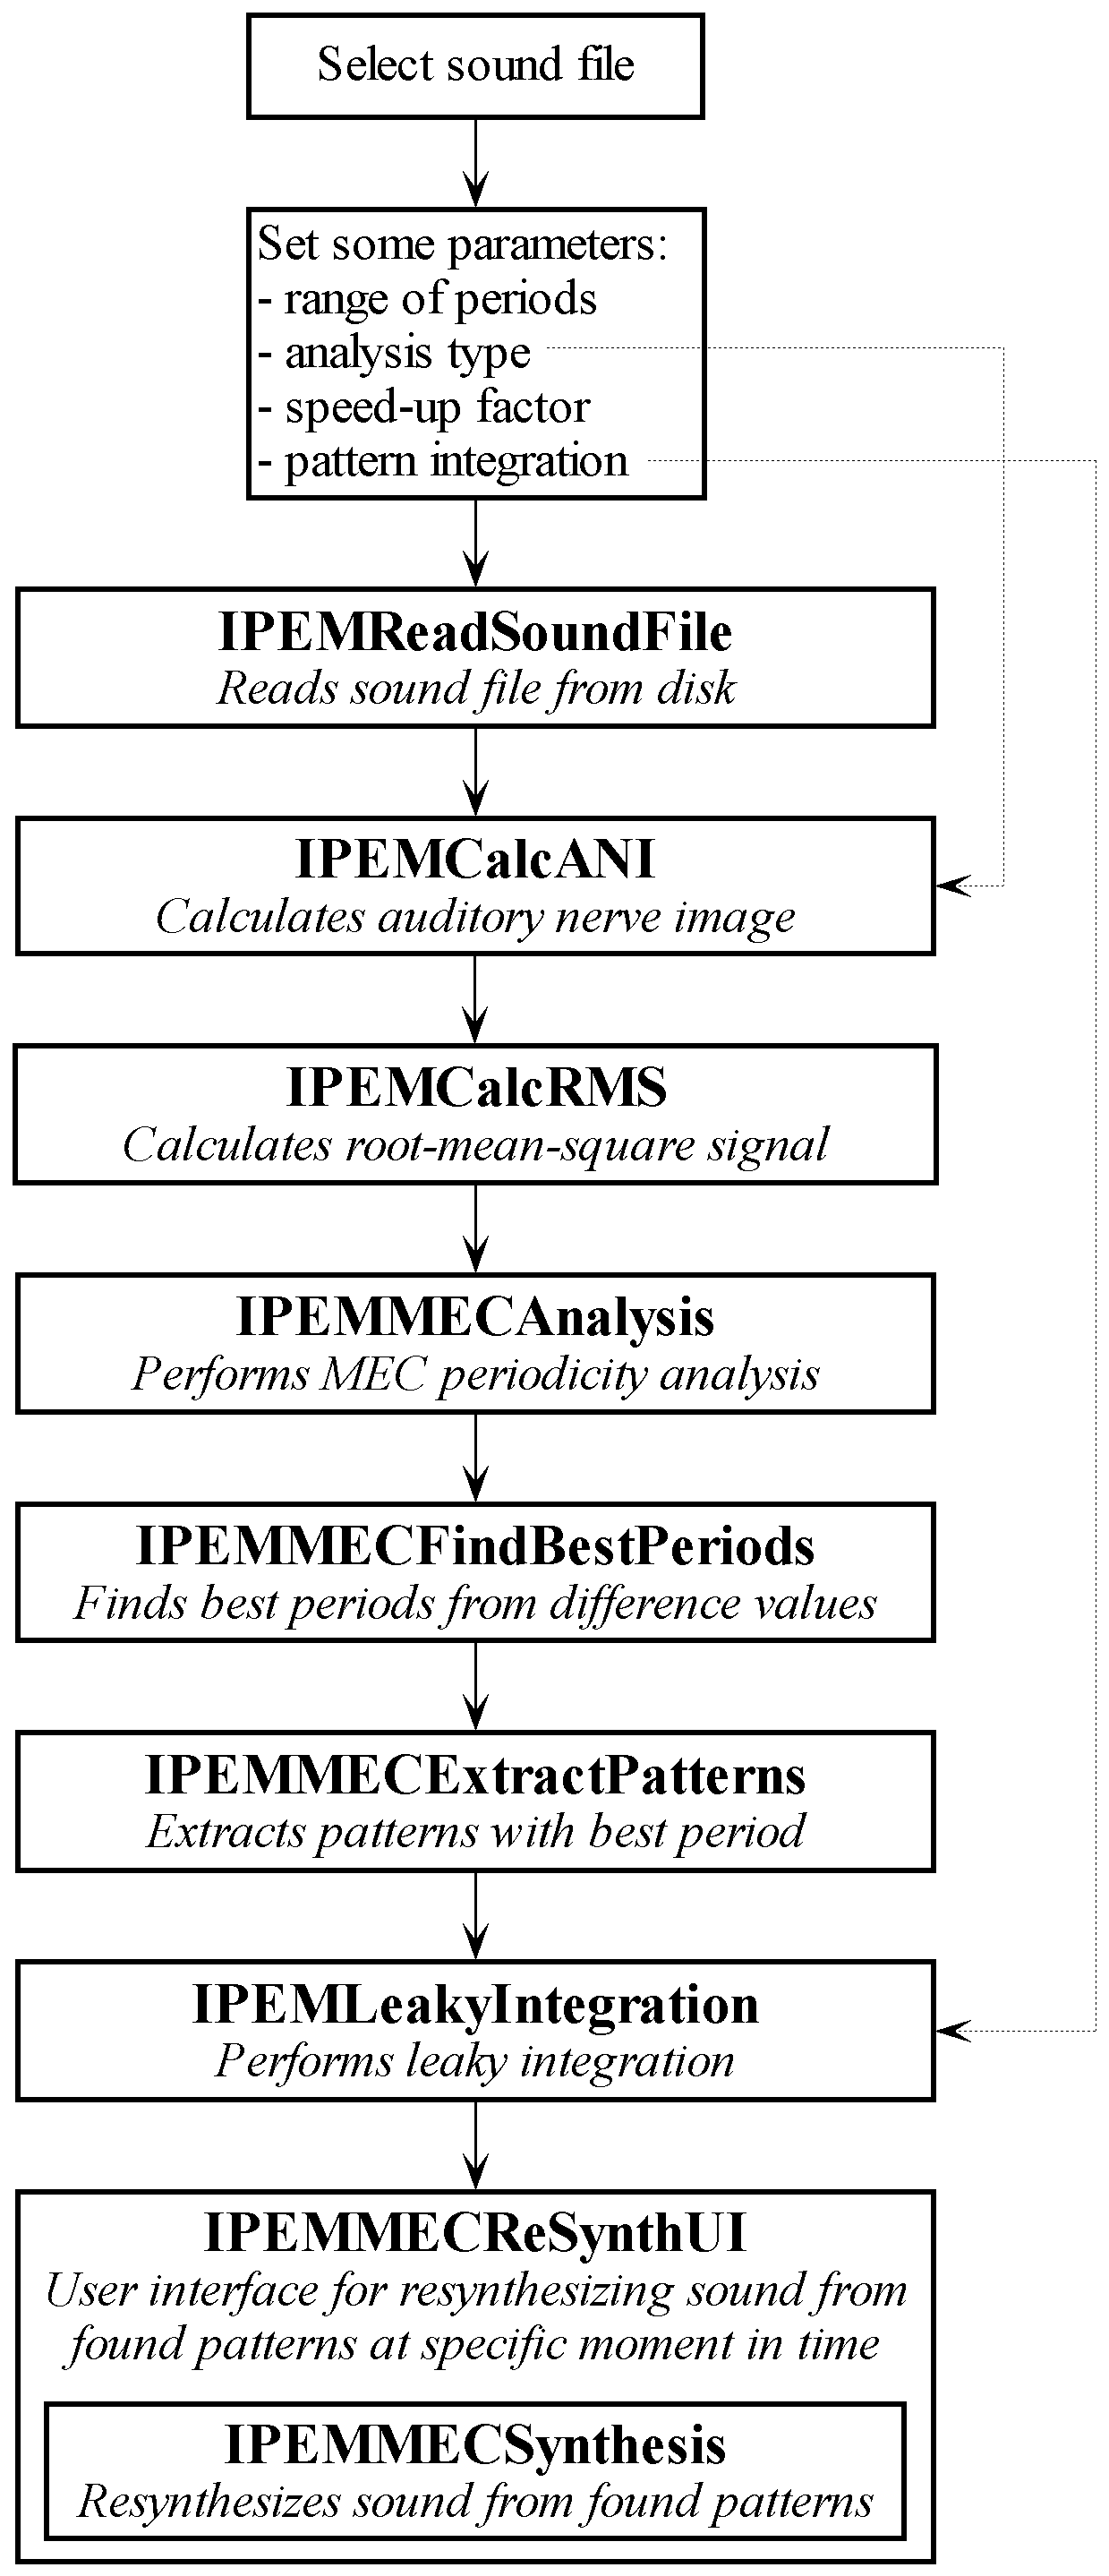
\includegraphics[width=8cm]{Graphics/IPEMDemoMECRhythmExtractionChart}
    \caption{Execution flow of IPEMDemoMECRhythmExtraction}
    \label{Fig:IPEMDemoMECRhythmExtractionChart}
\end{figure}

\begin{enumerate}
\item
    First of all, the user has to select the sound file he/she
    wants to analyze.\\
    Three example sound files are located in the directory containing
    the demo:
    \begin{itemize}
    \item Example 1: \IPEMSound{Sounds/BartokScherzoSuiteOp14.wav}{BartokScherzoSuiteOp14.wav}\\
        This is a short fragment from the beginning of the second movement "Scherzo"\\
        from "Suite op. 14" by B\'{e}la Bart\'{o}k (piano).
    \item Example 2: \IPEMSound{Sounds/TomWaitsBigInJapan.wav}{TomWaitsBigInJapan.wav}\\
        This is an excerpt from "Big in Japan" taken from "Mule Variations" by Tom Waits
        (voice, bass, drums, electric guitar).
    \item Example 3: \IPEMSound{Sounds/PhotekTheLightening.wav}{PhotekTheLightening.wav}\\
        This is a short fragment from "The Lightening (Digital Remix)" by Photek
        (electronic, drum and bass).
    \end{itemize}

\item
    Next, a few choices have to be made for setting the analysis parameters:
    \begin{itemize}
    \item Period range\\
        Specify the range of periods for which periodicity should be
        checked. For rhythmic patterns reasonable values are from 0.050 to 5
        seconds. The bigger the range, the more periods will be checked, so
        the slower the analysis will be.
    \item Type of analysis\\
        Finding the "best periods" can be done in three ways:
        \begin{itemize}
        \item using the difference values calculated from the RMS of
        the sound signal itself: this yields a single "best period" at
        each moment in time
        \item using the summed difference values (over all channels) calculated from the RMS of
        the ANI: this yields a single "best period" for all channels
        together at each moment in time
        \item using the difference values calculated from the RMS of
        the ANI separately for each channel: this yields a "best period" for each channel at each moment in
        time
        \end{itemize}
    \item Speed-up factor\\
        Instead of calculating difference values for every sample in the RMS
        signal, you can specify a speed-up factor n (a positive
        integer) so that values are calculated only every n samples.
    \item Pattern integration\\
        After extracting the patterns using the found best period
        at a certain moment, the patterns can be integrated over
        time. This can be done to decrease the effect of small local
        variations.
    \end{itemize}

\item
    Then, the sound file is read and the RMS is calculated with
    \hyperlink{FuncRef:IPEMCalcRMS}{IPEMCalcRMS}, either on the
    auditory nerve image of the sound, or on the sound itself,
    depending on what was specified in the previous step. The
    auditory nerve image is calculated with
    \hyperlink{FuncRef:IPEMCalcANI}{IPEMCalcANI} using 10 bands
    with a bandwidth of 1.5 critical band units (cbu), starting
    at 3 cbu. This corresponds to center frequencies of 215 Hz to
    3266 Hz.

\item
    The MEC algorithm then starts analyzing the RMS signal
    (\hyperlink{FuncRef:IPEMMECAnalysis}{IPEMMECAnalysis}) by calculating difference values.

\item
    Then the most prominent period(s) at each moment in time are selected.
    A figure with the best period(s) over time is generated (for RMS
    of ANI, this is a multi-channel plot, for RMS of sound
    signal, this is a single-channel plot).

\item
    The results of the previous analysis (the best period(s) at each
    moment) is then used to extract the corresponding pattern(s) from
    the RMS signal with
    \hyperlink{FuncRef:IPEMMECExtractPatterns}{IPEMMECExtractPatterns}.\\
    Depending on the specified parameters, these patterns can be
    further integrated over time with
    \hyperlink{FuncRef:IPEMLeakyIntegration}{IPEMLeakyIntegration}.

\item
    Finally, resynthesis of the extracted patterns can be done
    using \hyperlink{FuncRef:IPEMMECReSynthUI}{IPEMMECReSynthUI} (which
    calls
    \hyperlink{FuncRef:IPEMMECSynthesis}{IPEMMECSynthesis}
    internally.\\
    The presented user interface consists of two figures: one is
    the figure showing the (multi-channel) best periods over time
    and the other is a "control palette" with some push buttons.\\
    In the first figure, a moment in time (and a specific
    channel) can be selected by pressing the left mouse button.\\
    Once this selection is made, a resynthesis can be done by
    pressing the "Resynthesize for selected time" button. This
    button is only enabled when the selected time is different
    from the time for which resynthesis was last done.\\
    In order to evaluate the resynthesized sound, it is combined
    with the original sound into a stereo sound file, where the
    left channel plays the original sound and the right channel
    plays the synthesized sound. By pressing the "Play all
    channels" button, the last resynthesized sounds for all
    channels are played together, while the "Play selected
    channel" only plays the selected channel.\\
    Pressing a key (rather than clicking with the mouse) in the
    first figure ends the resynthesis.\\
    Figure \ref{Fig:MECDemoUI} shows a snapshot of the
    resynthesis user interface.

\end{enumerate}

\begin{figure}
    \centering
    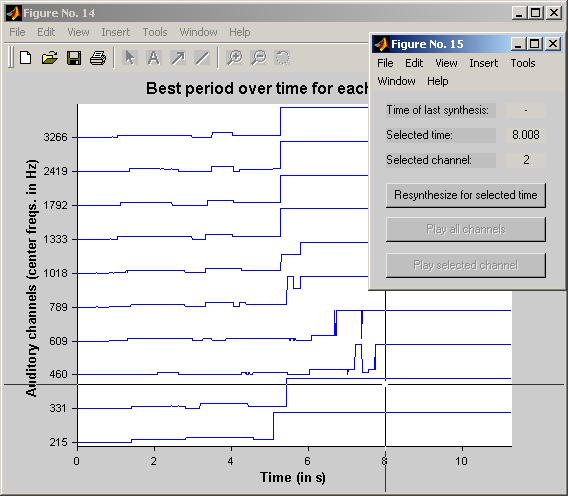
\includegraphics[width=\IPEMDefaultFigureWidth]{Graphics/MECDemoPhotekTheLighteningUI}
    \caption{Resynthesis user interface}
    \label{Fig:MECDemoUI}
\end{figure}

\subsubsection*{One run demo function}

This demo function does essentially the same as the above
interactive demo, but it runs without any user intervention. All
parameters have to be specified when calling the function, and
then everything is calculated in one go, without interruption.

Figure \ref{Fig:IPEMDemoStartMEC} shows the execution flow of
IPEMDemoStartMEC.

\begin{figure}[h]
    \centering
    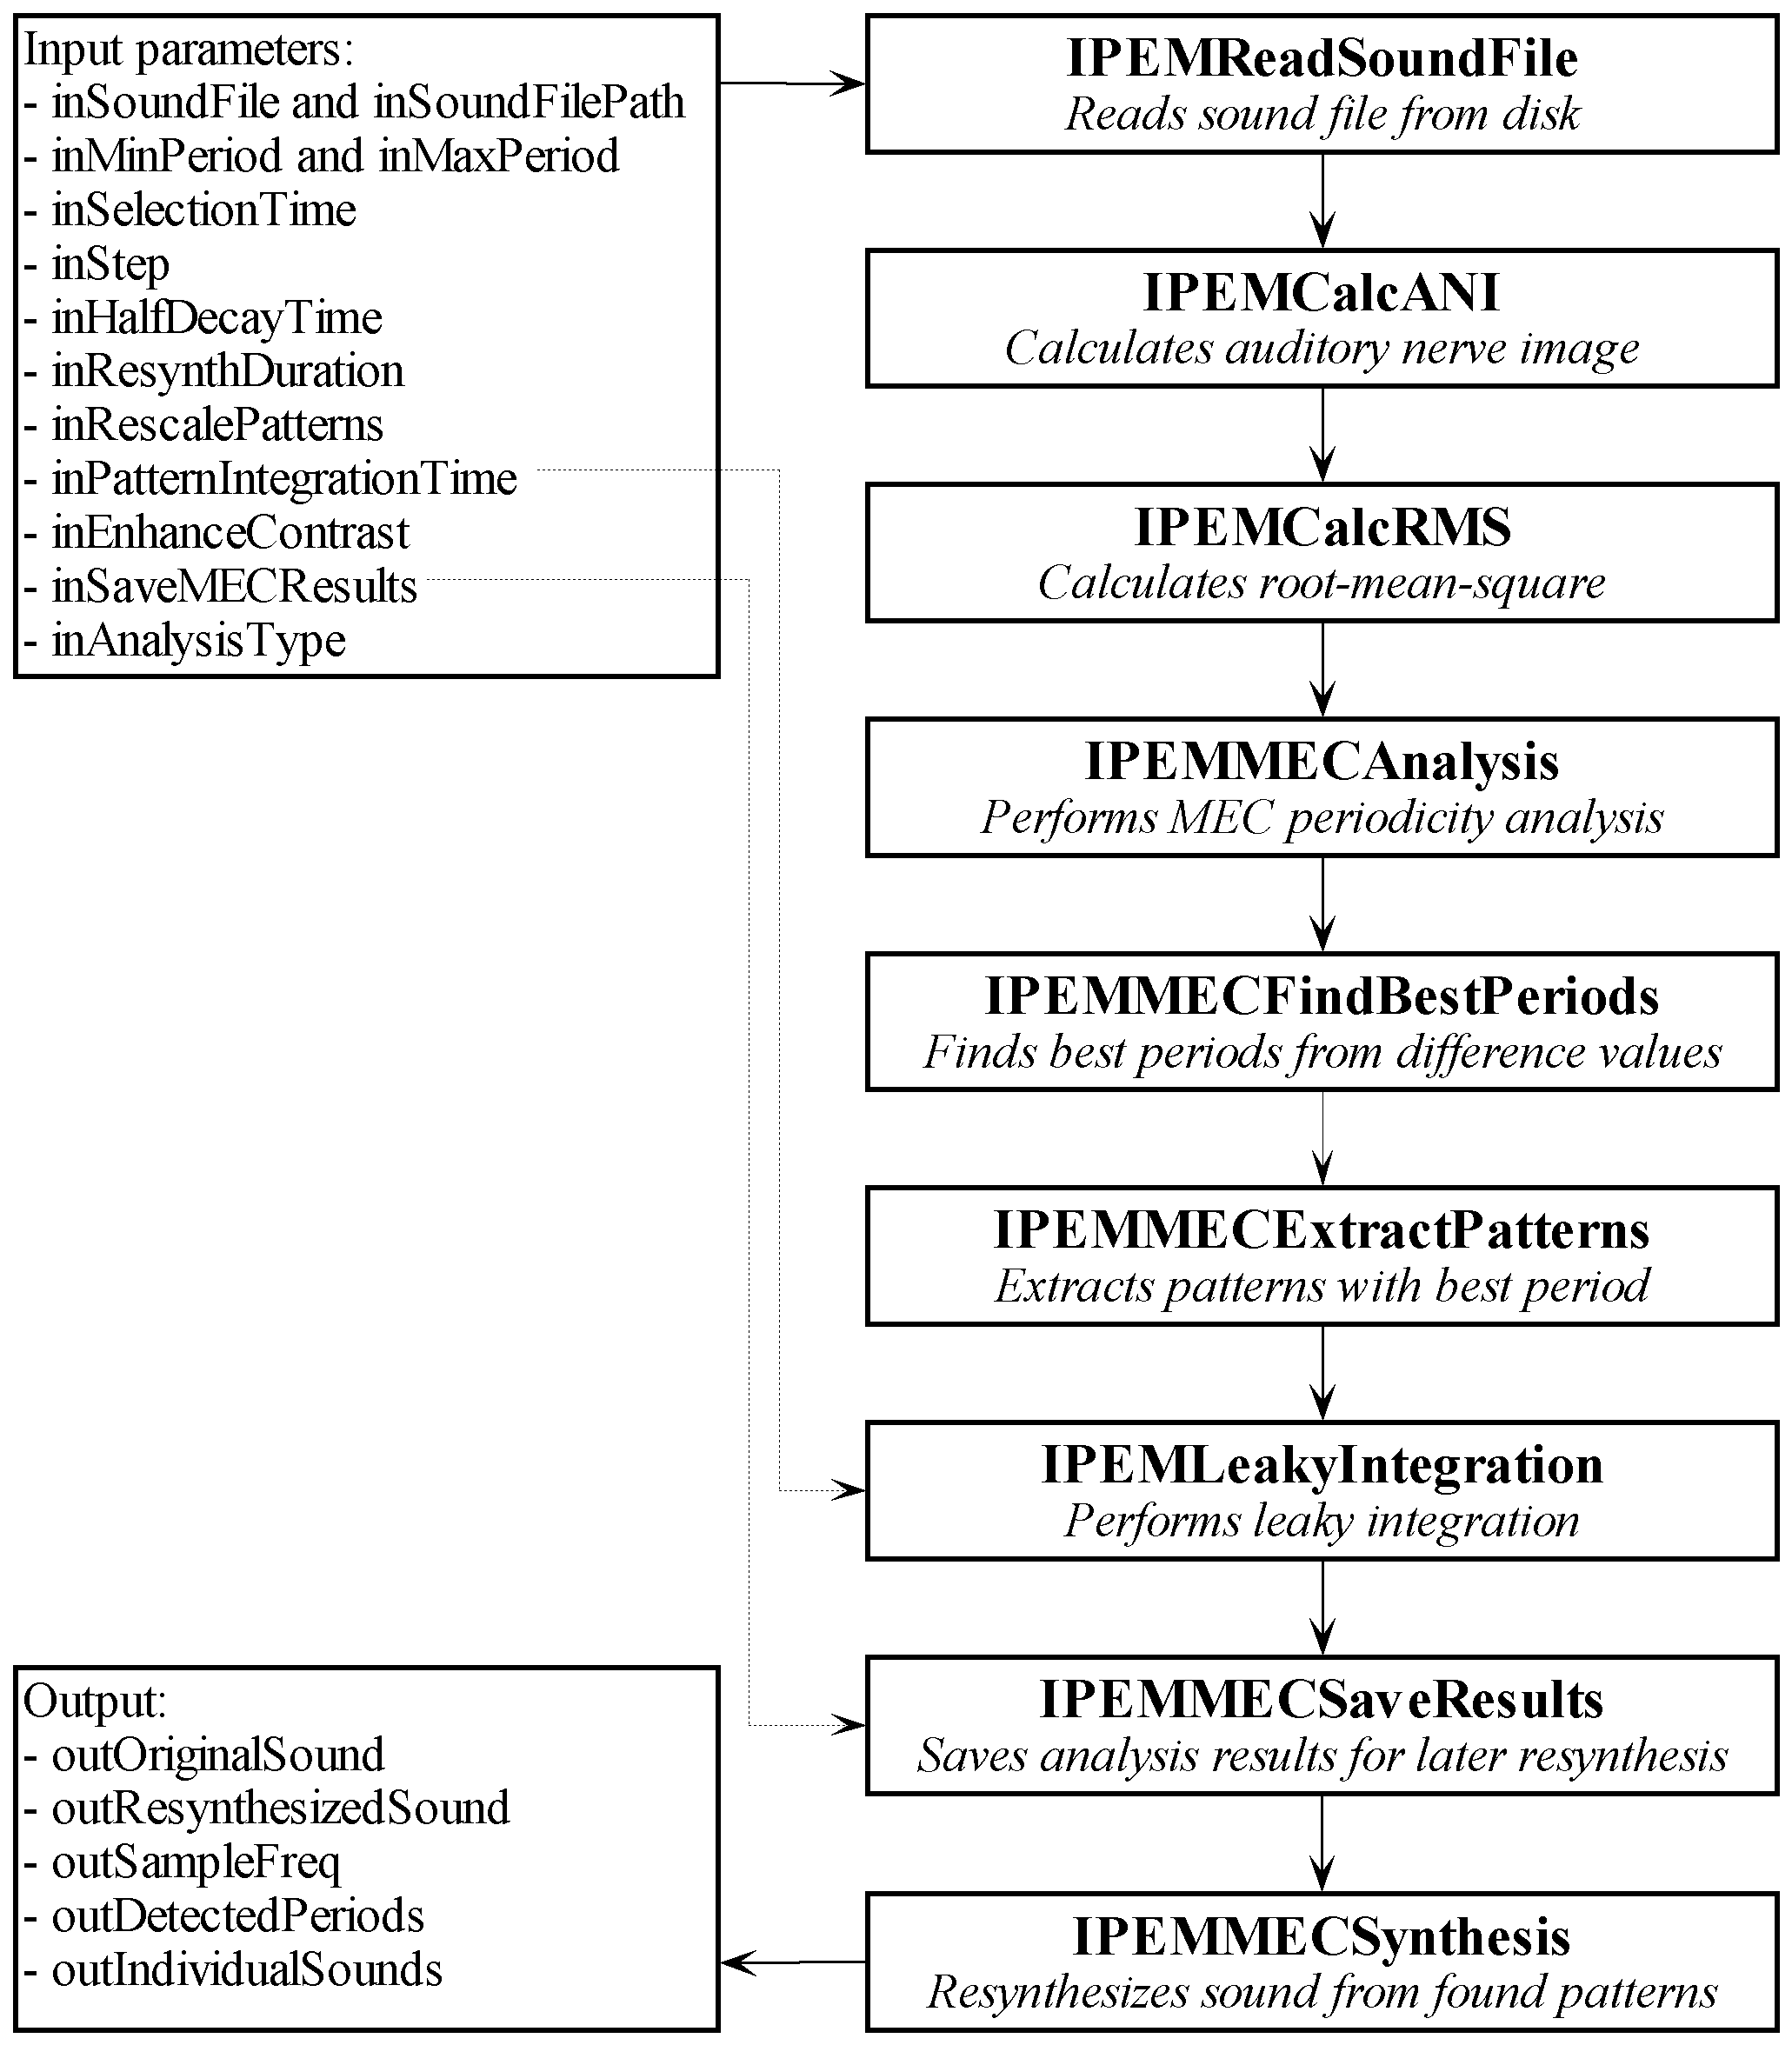
\includegraphics[width=\IPEMDefaultFigureWidth]{Graphics/IPEMDemoStartMEC}
    \caption{Execution flow of IPEMDemoStartMEC}
    \label{Fig:IPEMDemoStartMEC}
\end{figure}

The results of the analysis can be saved to a .mat file so that
resynthesis can be performed at a time later using either
\hyperlink{FuncRef:IPEMMECSynthesis}{IPEMMECSynthesis} or
\hyperlink{FuncRef:IPEMMECReSynthUI}{IPEMMECReSynthUI} after
reloading the data.


\subsubsection*{Remarks about the method of "resynthesis"}

The resynthesis is done by amplitude modulation of specific noise
bands with the extracted patterns. In case the RMS was calculated
on the auditory nerve image, the noise bands have a center
frequency equal to the center frequency of the corresponding
auditory channel. In case the RMS was calculated directly on the
sound signal, broad band noise is used. The resynthesized sound
pattern is then repeated until the total sound duration matches
that of the original sound.\\
Both are finally combined into a stereo sound where one channel
plays the original sound and the other plays the resynthesized sound.\\

Note that this "resynthesis" is just a "quick and dirty" way to
quickly hear the results of the pattern extraction. It assumes
that the entire sound is a constant repetition of the selected
pattern and this has a few important limitations:
\begin{enumerate}
\item drift\\
When the pattern is selected for the specified moment in time, it
is inserted before and after that moment as many times as needed
to obtain the total duration of the original sound. This means
that if there are small tempo fluctuations, the sound will only
match very well in the neighborhood of the selected moment in
time, but maybe not elsewhere. You might hear this "drifting" when
playing back the stereo sound.
\item gaps\\
This is a more extreme case of the above: when there is a gap in
the rhythmic flow (even if the tempo is constant), the
resynthesized sound will be out of sync with the original sound.
Again, only at the selected moment in time, there will be perfect
synchronization.
\item separated channels\\
When "separated channels" are used, a best period is found for
each channel, so it is perfectly possible that in the higher
channels a period was detected different from the one in the lower
channels. The resynthesis uses these patterns and you might thus
hear different patterns at the same time (each in a different
frequency range). This might be good for drum sequences where you
have different patterns for hihats and bass drum. If the pattern
lengths only differ slightly, again drift might be hearable.
\end{enumerate}


% --------------------------------------------------------------------------------
\subsection{Results and discussion}
% --------------------------------------------------------------------------------

\subsubsection*{Sound example 1}

Figure \ref{Fig:MECBartokExample} shows graphic results for the
sound example
\IPEMSound{Sounds/BartokScherzoSuiteOp14.wav}{BartokScherzoSuiteOp14.wav}.\\

The \emph{top left graph} shows the original sound and the
calculated RMS signal levels. It is this RMS signal that is
examined by the MEC analysis for repeating patterns.\\

The \emph{top right graph} shows the difference values calculated
by the MEC analysis together with the best period (corresponding
to the period for which the difference value is minimal).\\

The \emph{lower left graph} shows the effect of pattern
integration. A leaky integration with half decay time 0.5 s was
used, which has the effect that small differences between
successive patterns are eliminated in favor of a more stable
pattern. Of course, this also "flattens" the detected patterns and
"smears" them over time, so an appropriate choice for the half
decay time should be chosen.\\

The \emph{lower right graph} shows the graphical interface that
can be used for resynthesizing the rhythm starting from the
extracted patterns at a selected moment in time. To hear the
result of this "rhythm resynthesis" for this example, you can
listen to the following sound:
\begin{itemize}
\item[] - \IPEMSound{Sounds/MECDemoBartokScherzoSuiteOp14ReSynthAll.wav}{Resynthesis from RMS of sound}
\end{itemize}
This sound was resynthesized using repetitions of the pattern
extracted at 4.5 s, where a best period of 1.604 s was detected.
The left channel plays the original sound, while the right channel
plays the synthesized sound. The patterns in each channel were
rescaled between 0 and 1 (this is a parameter
of \hyperlink{FuncRef:IPEMMECExtractPatterns}{IPEMMECExtractPatterns}).\\

The signals of the synthesized sounds were further processed using
a third power function to enhance contrast in the sounds
($s_{enh}(t) = s(t)^3$, where $s(t)$ was first normalized between
-1 and 1). This is a parameter of the base function for
resynthesis of MEC results \hyperlink{FuncRef:IPEMMECSynthesis}{IPEMMECSynthesis}.\\


\subsubsection*{Sound example 2}

Figure \ref{Fig:MECTomWaitsExample} shows graphic results for the
sound example \IPEMSound{Sounds/TomWaitsBigInJapan.wav}{TomWaitsBigInJapan.wav}.\\

The \emph{top left graph} shows the auditory nerve image (ANI)
calculated for 10 bands having a configuration as explained in the interactive demo.\\

The RMS signal of this ANI is shown in the \emph{top right graph}.
It is this signal that is examined by the MEC analysis for repeating patterns.\\

The \emph{middle left graph} then shows the difference values
calculated by the MEC analysis together with the best period
(corresponding to the period for which the difference value is
minimal). Difference values were calculated for each channel and
then summed together to result in the shown overall difference
values.\\

The \emph{middle right graph} shows the effect of  pattern
integration. Again, a leaky integration with half decay time 0.5 s
was used.\\

The \emph{lower left graph} again shows the graphical interface
that can be used for resynthesizing the rhythm starting from the
extracted patterns at a selected moment in time. This resynthesis
can be done for each channel separately, but they all use the same
"best period" . To hear some examples of resynthesis, you can
listen to the following sounds:
\begin{itemize}
\item[] - \IPEMSound{Sounds/MECDemoTomWaitsBigInJapanReSynthANIAll.wav}{Resynthesis for all channels}
\item[] - \IPEMSound{Sounds/MECDemoTomWaitsBigInJapanReSynthANICh2.wav}{Resynthesis for channel 2}
\item[] - \IPEMSound{Sounds/MECDemoTomWaitsBigInJapanReSynthANICh9.wav}{Resynthesis for channel 9}
\end{itemize}
The sounds were in this case resynthesized using repetitions of
the patterns extracted in each channel at around 12 s, where a
best period of 2.133 s was detected. The left channel plays the
original sound, while the right channel plays the synthesized
sound. Again, re-scaling of patterns and contrast enhancement for
the synthesized sounds was applied.


\subsubsection*{Sound example 3}

Figure \ref{Fig:MECPhotekExample} shows graphic results for the
sound example
\IPEMSound{Sounds/PhotekTheLightening.wav}{PhotekTheLightening.wav}.\\

The \emph{top left graph} shows the auditory nerve image (ANI)
calculated for 10 bands having a configuration as explained in the interactive demo.\\

The RMS signal of this ANI is shown in the \emph{top right graph}.
It is this signal that is examined by the MEC analysis for repeating patterns.\\

The \emph{middle left graph} then shows the difference values
calculated by the MEC analysis together with the best period
(corresponding to the period for which the difference value is
minimal). These results are of obtained for each channel, but here
only the values for channel 5 are shown as an example. In contrast
to the previous example where the difference values were summed
together, here each channel is treated separately.\\

The \emph{middle right graph} shows the best periods over time for
all channels. No absolute values are shown, but rather an overview
of the stability of the detected periods.\\

The \emph{lower left graph} shows the effect of  pattern
integration. As in the other examples, a leaky integration with
half decay time 0.5 s was used.\\

The \emph{lower right graph} again shows the graphical
"resynthesis" interface, this time with (possibly) different best
periods per channel. The following sounds were synthesized from
the extracted patterns:
\begin{itemize}
\item[] - \IPEMSound{Sounds/MECDemoPhotekTheLighteningReSynthANIAll.wav}{Resynthesis for all channels}
\item[] - \IPEMSound{Sounds/MECDemoPhotekTheLighteningReSynthANICh2.wav}{Resynthesis for channel 2}
\item[] - \IPEMSound{Sounds/MECDemoPhotekTheLighteningReSynthANICh9.wav}{Resynthesis for channel 9}
\end{itemize}
These sounds were resynthesized using repetitions of the patterns
extracted in each channel at around 8 s. Left and right channel
again play original and resynthesized sounds respectively, and
pattern scaling and "contrast" enhancement were applied as well.


% Figures for the examples

\begin{figure}[p]
    \begin{tabular}{cc}
        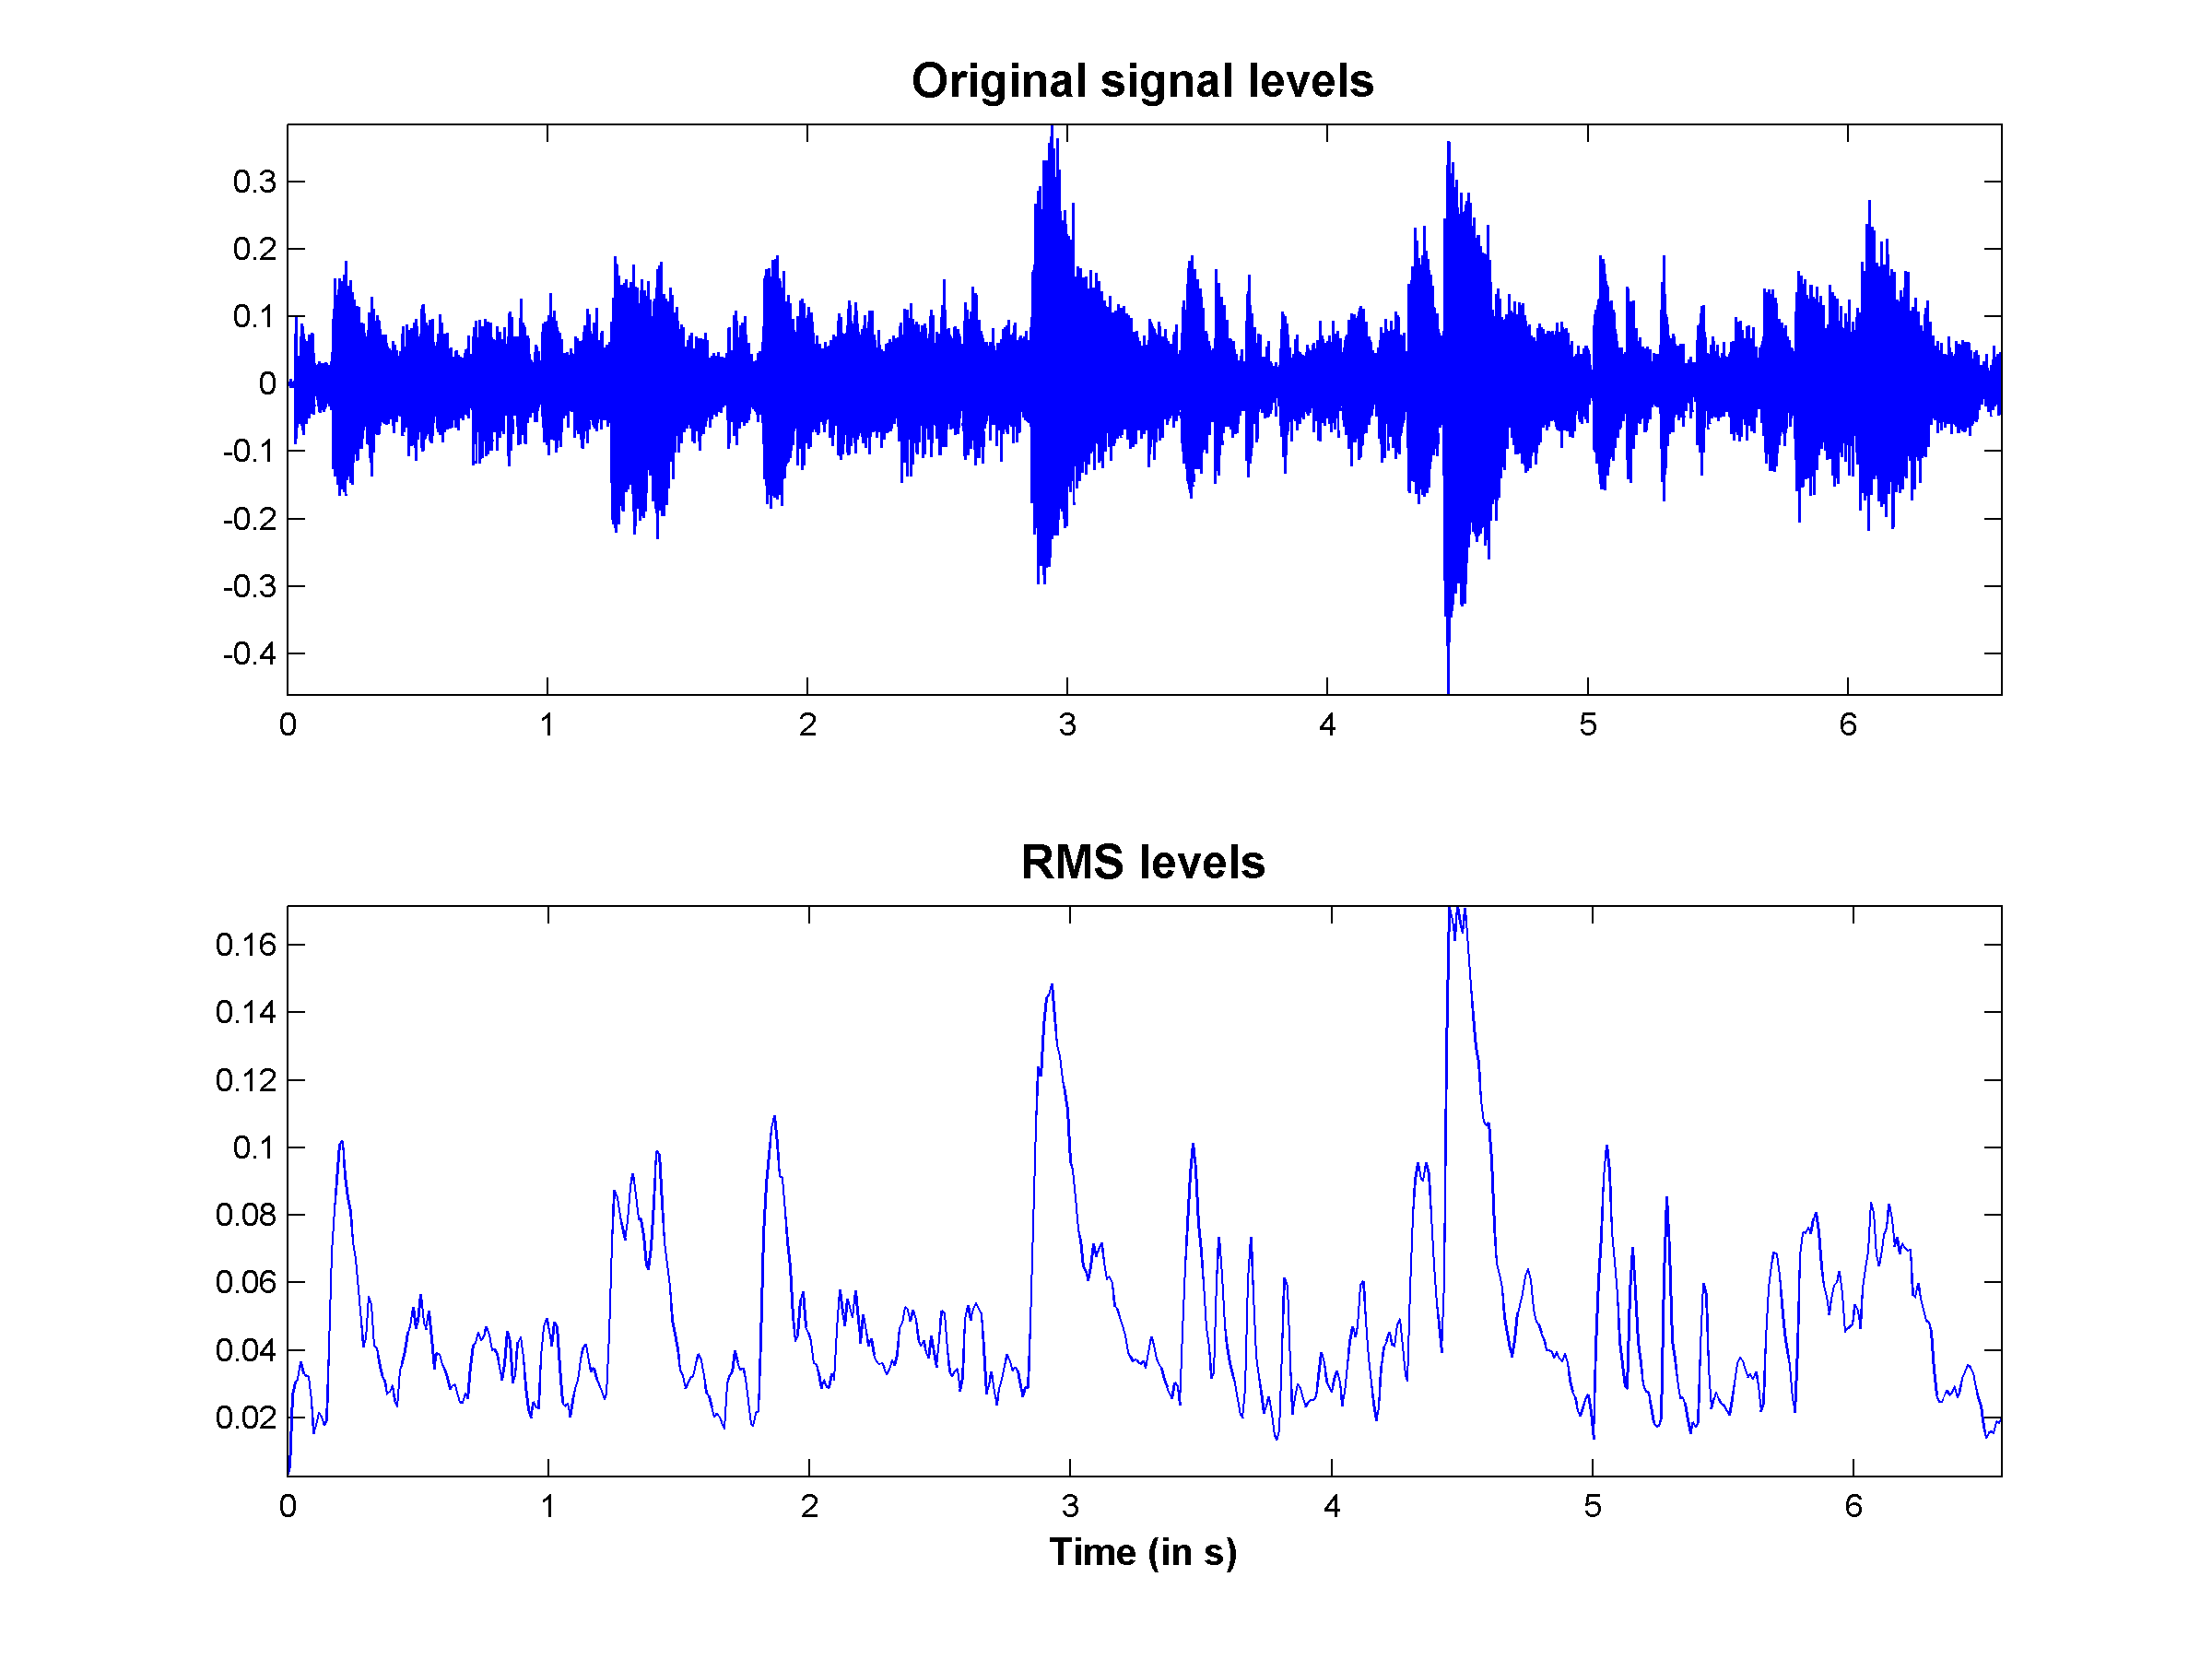
\includegraphics[width=7.5cm]{Graphics/MECDemoBartokScherzoSuiteOp14RMS} & 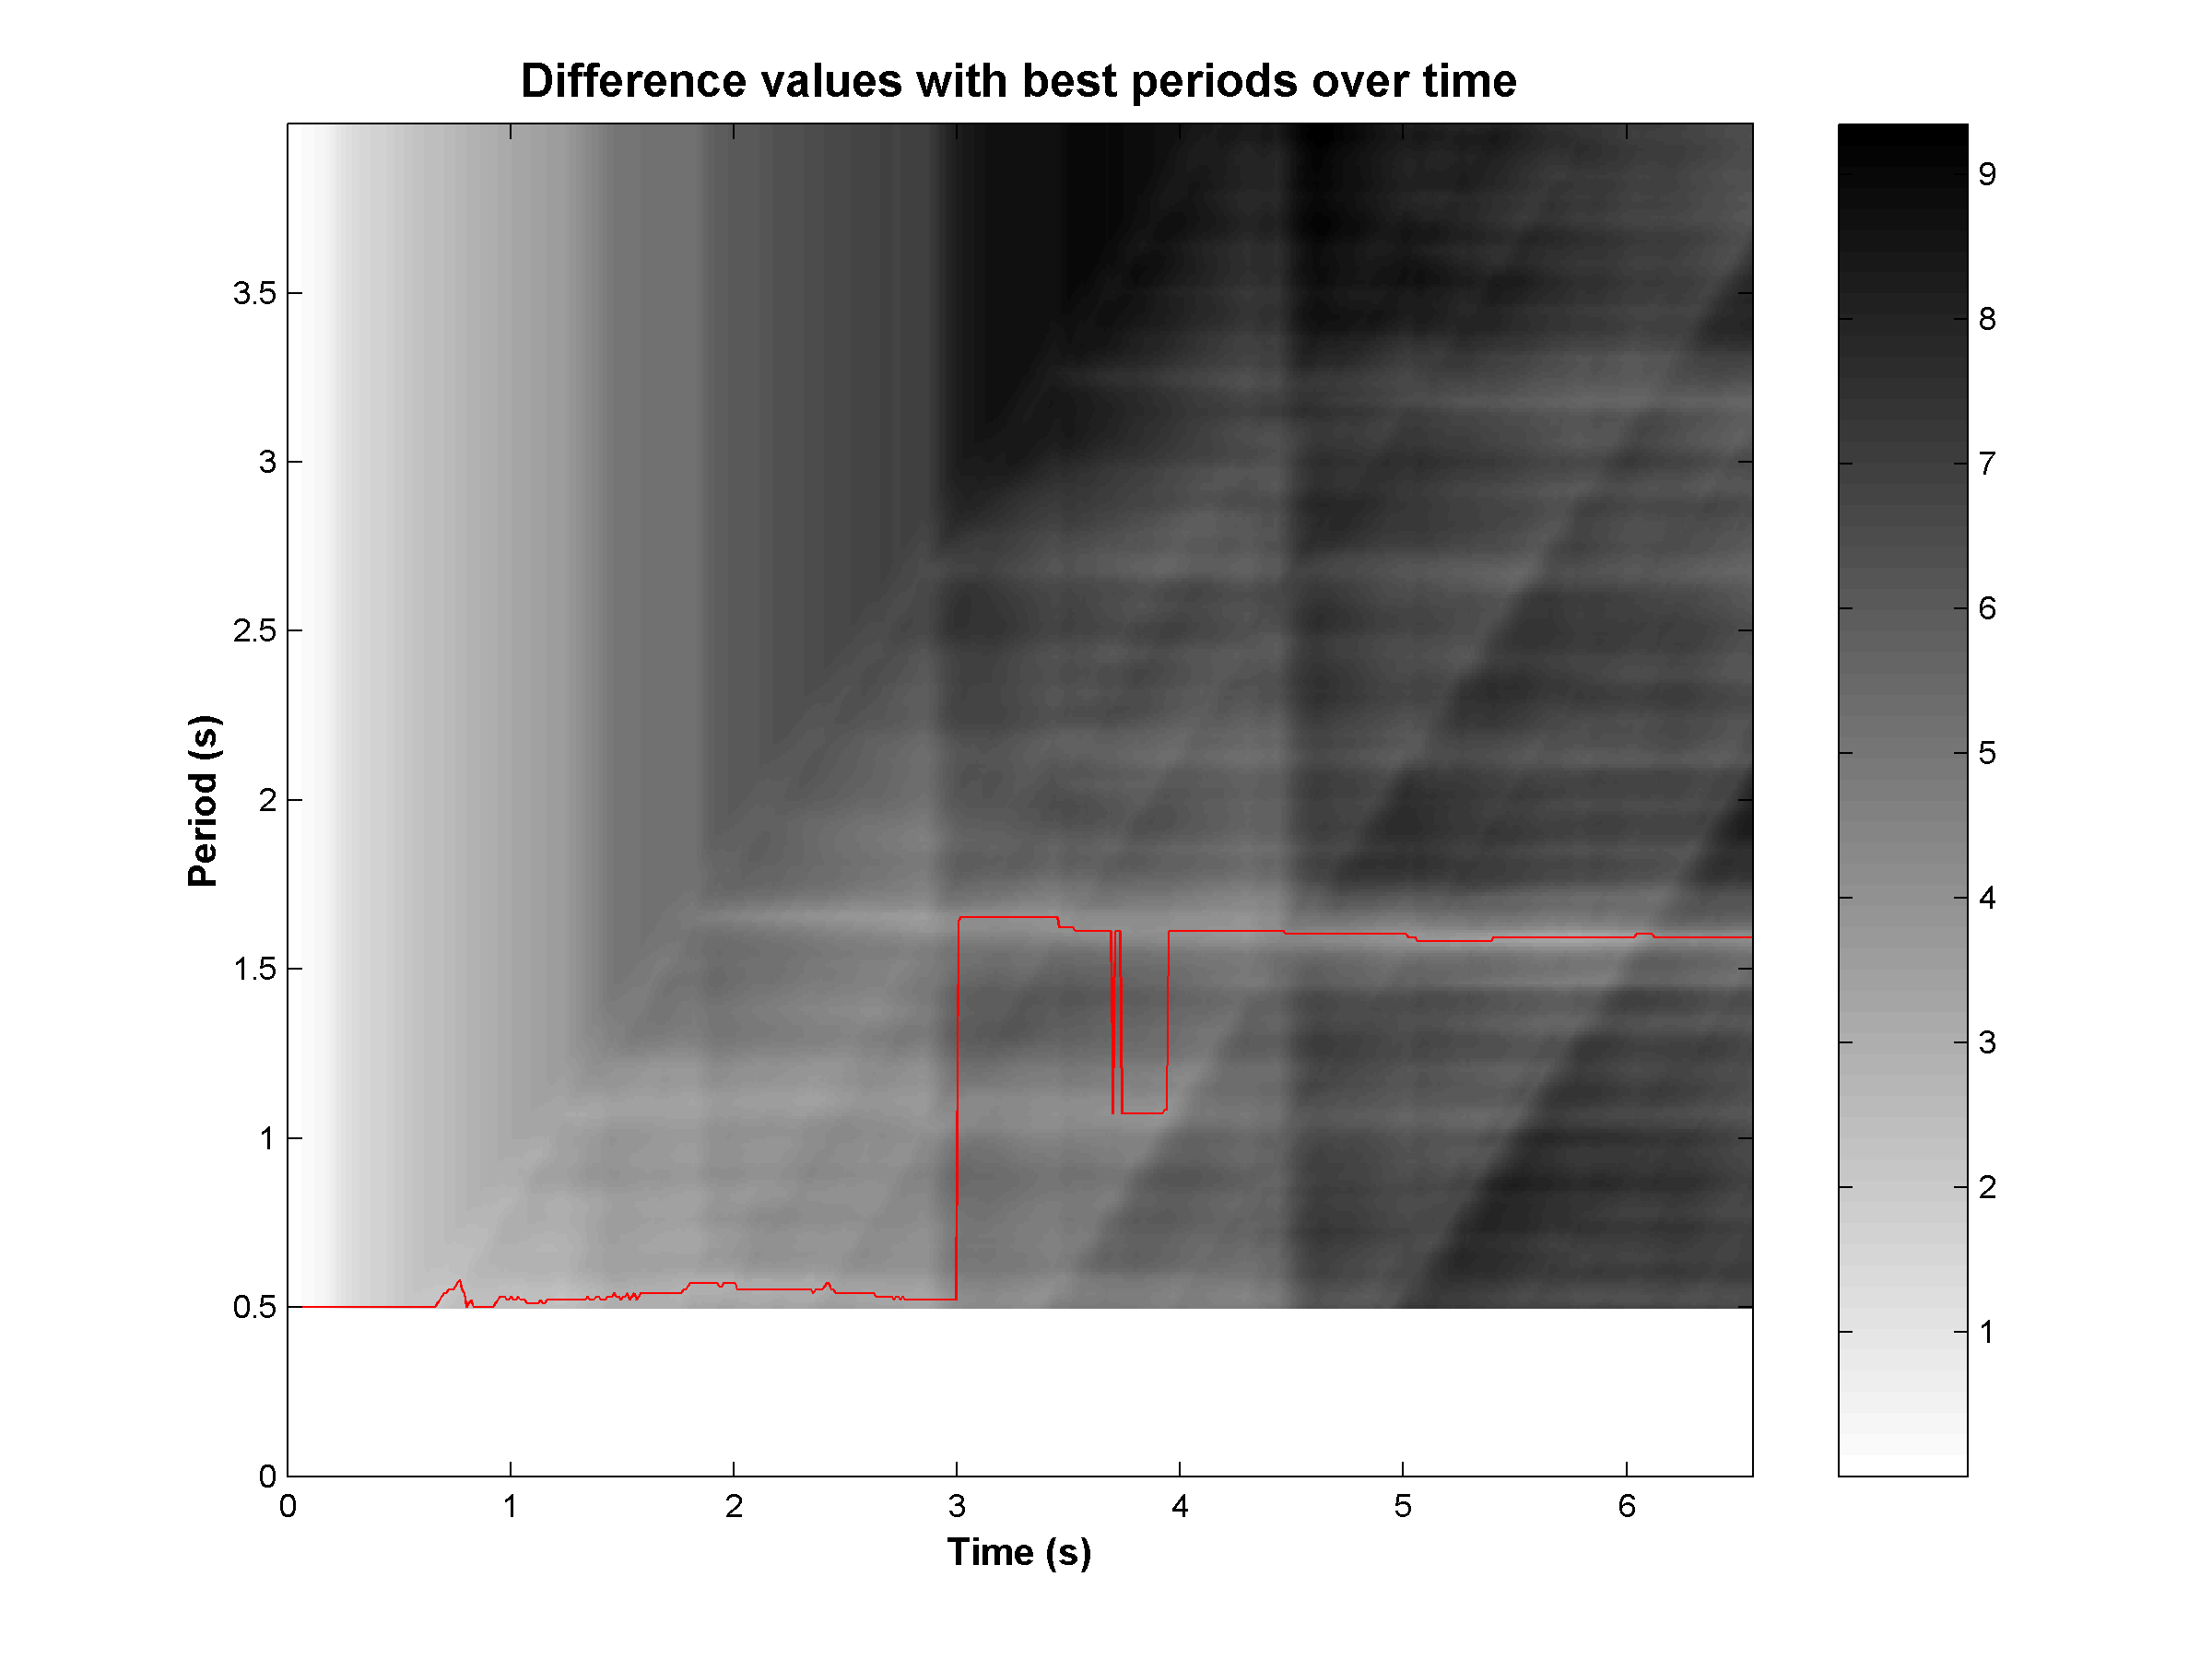
\includegraphics[width=7.5cm]{Graphics/MECDemoBartokScherzoSuiteOp14Values}\\
        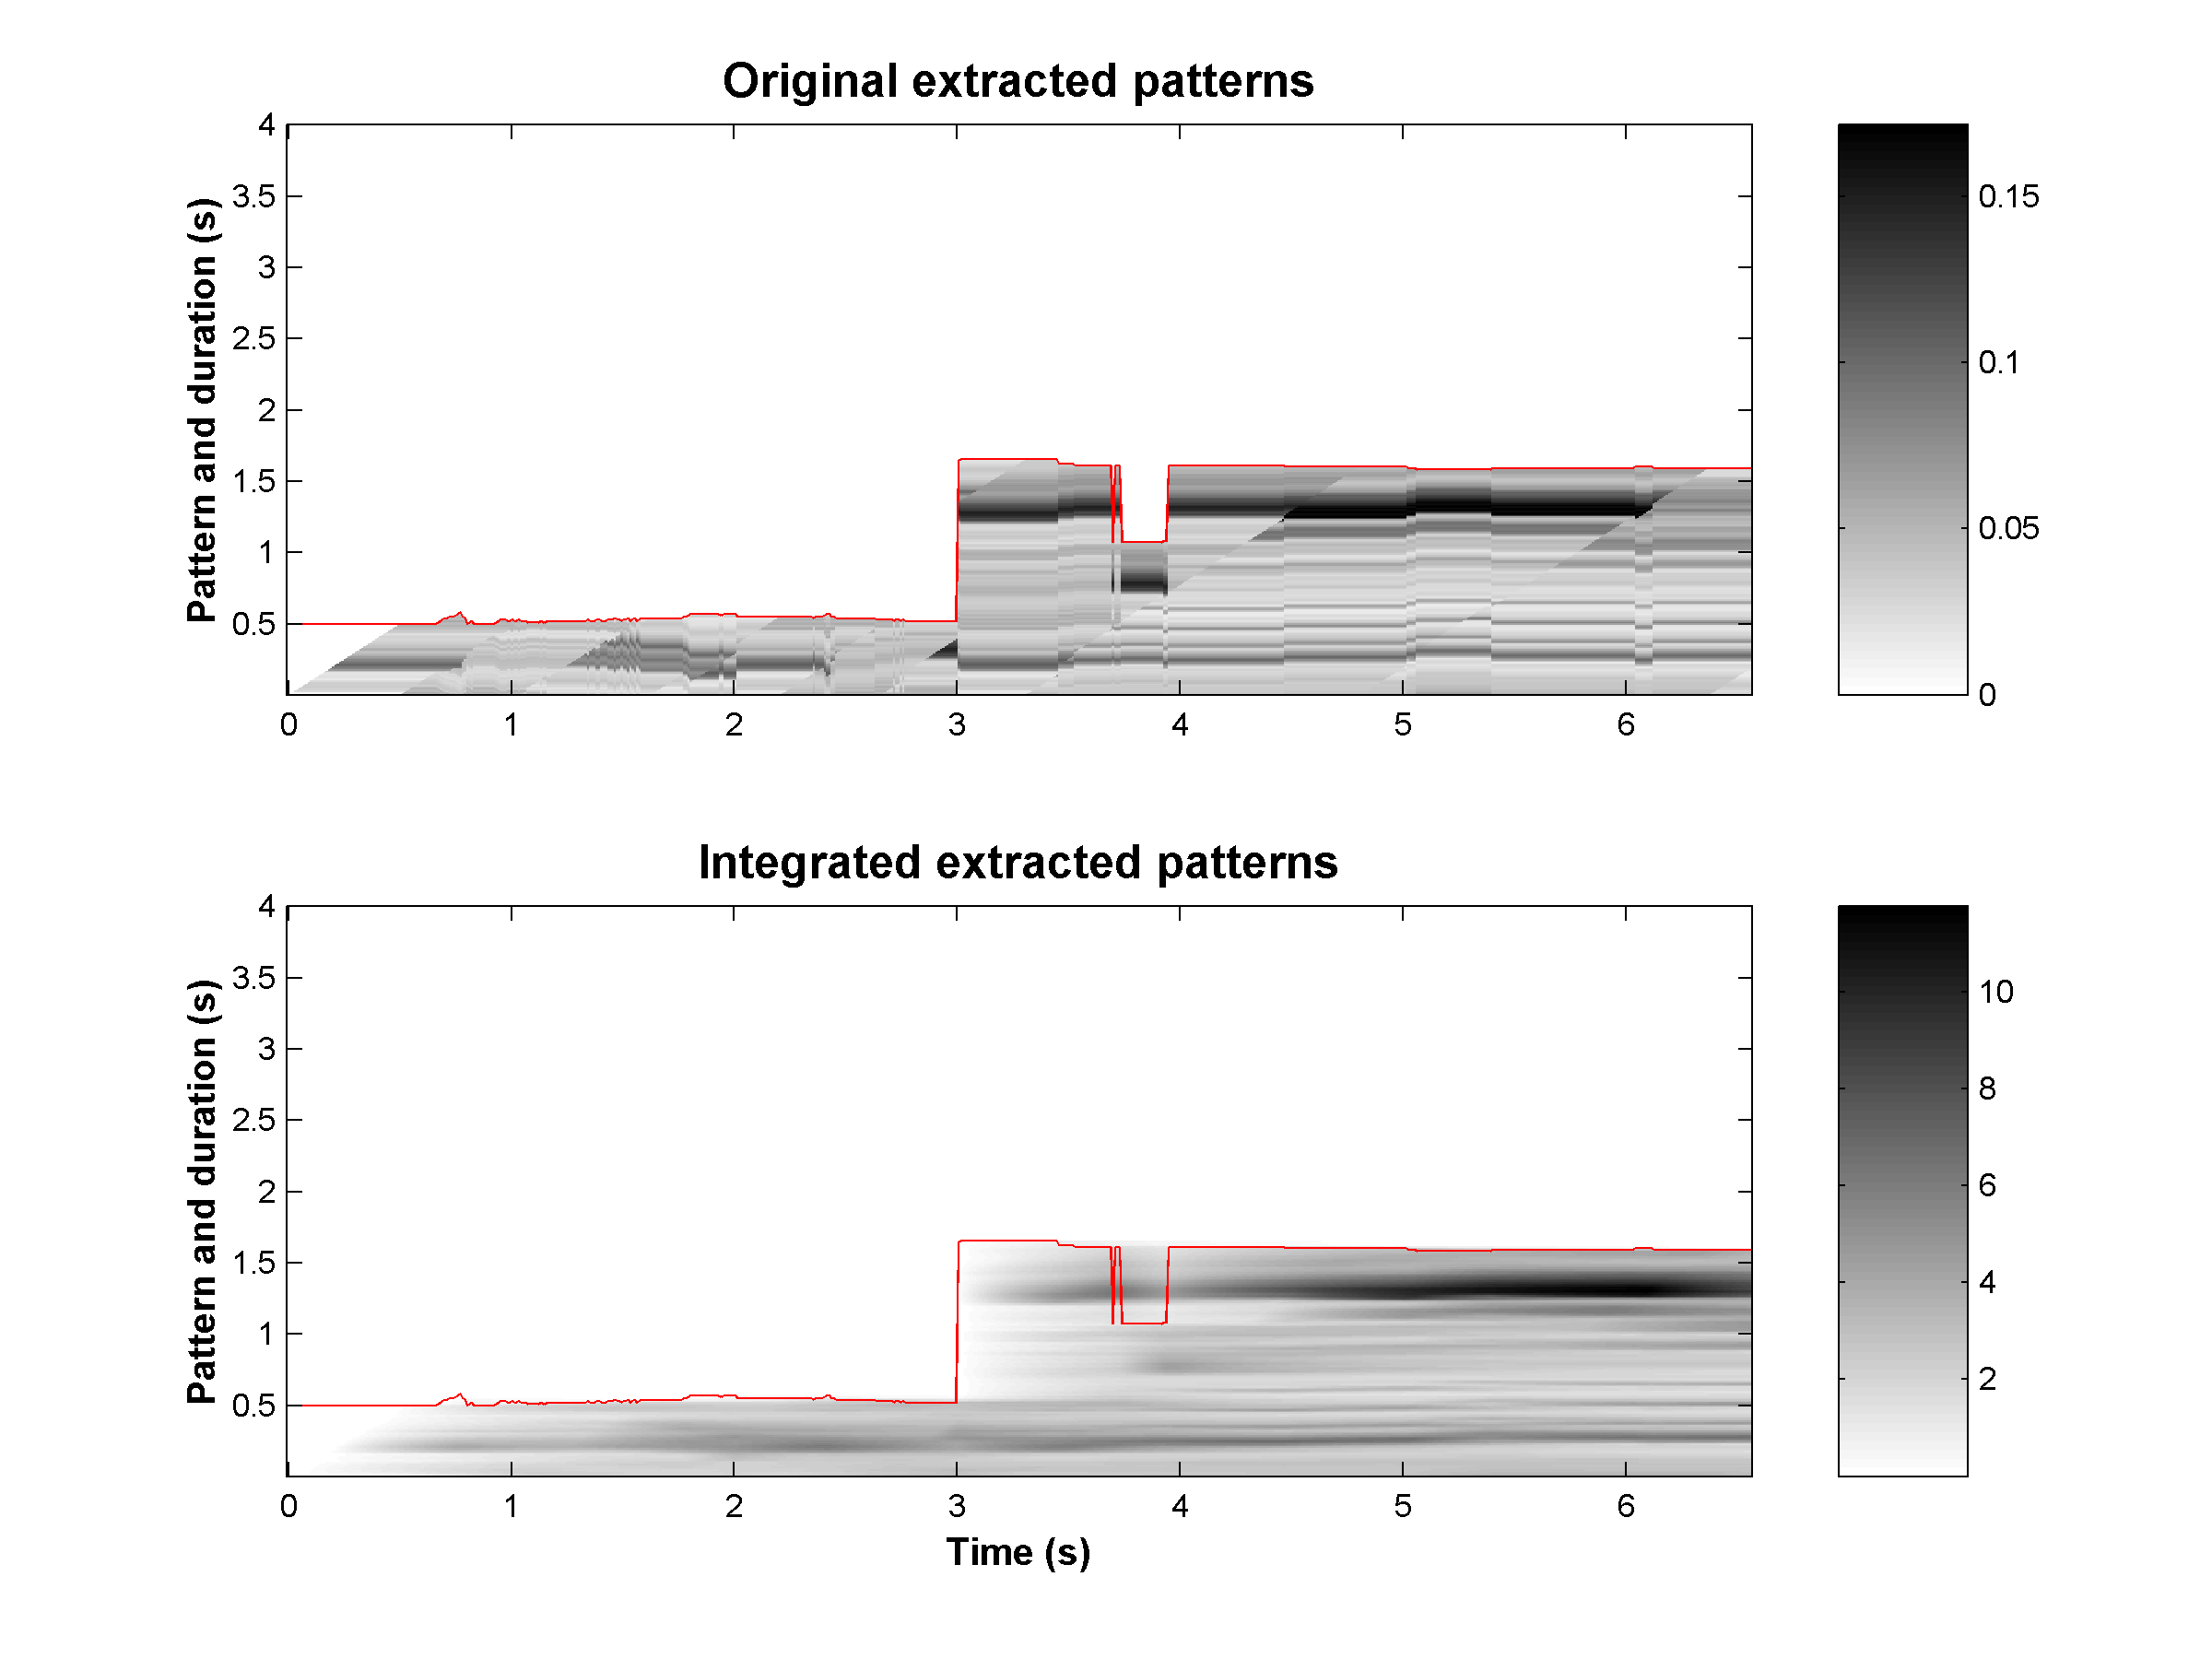
\includegraphics[width=7.5cm]{Graphics/MECDemoBartokScherzoSuiteOp14IntegrPatt} & 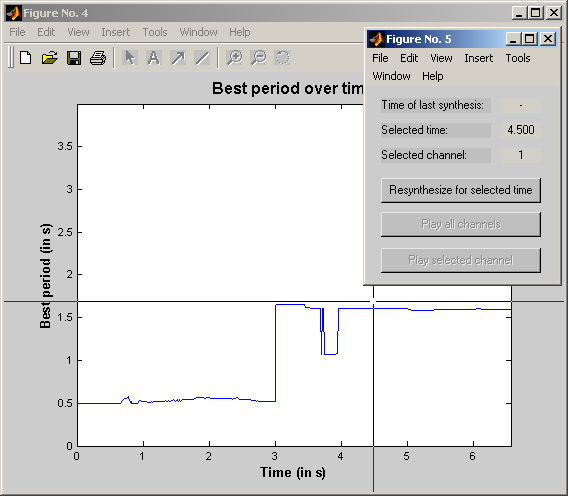
\includegraphics[width=7.5cm]{Graphics/MECDemoBartokScherzoSuiteOp14UI}\\
    \end{tabular}
    \caption{Results for BartokScherzoSuiteOp14.wav}
    \label{Fig:MECBartokExample}
\end{figure}

\begin{figure}[p]
    \begin{tabular}{cc}
        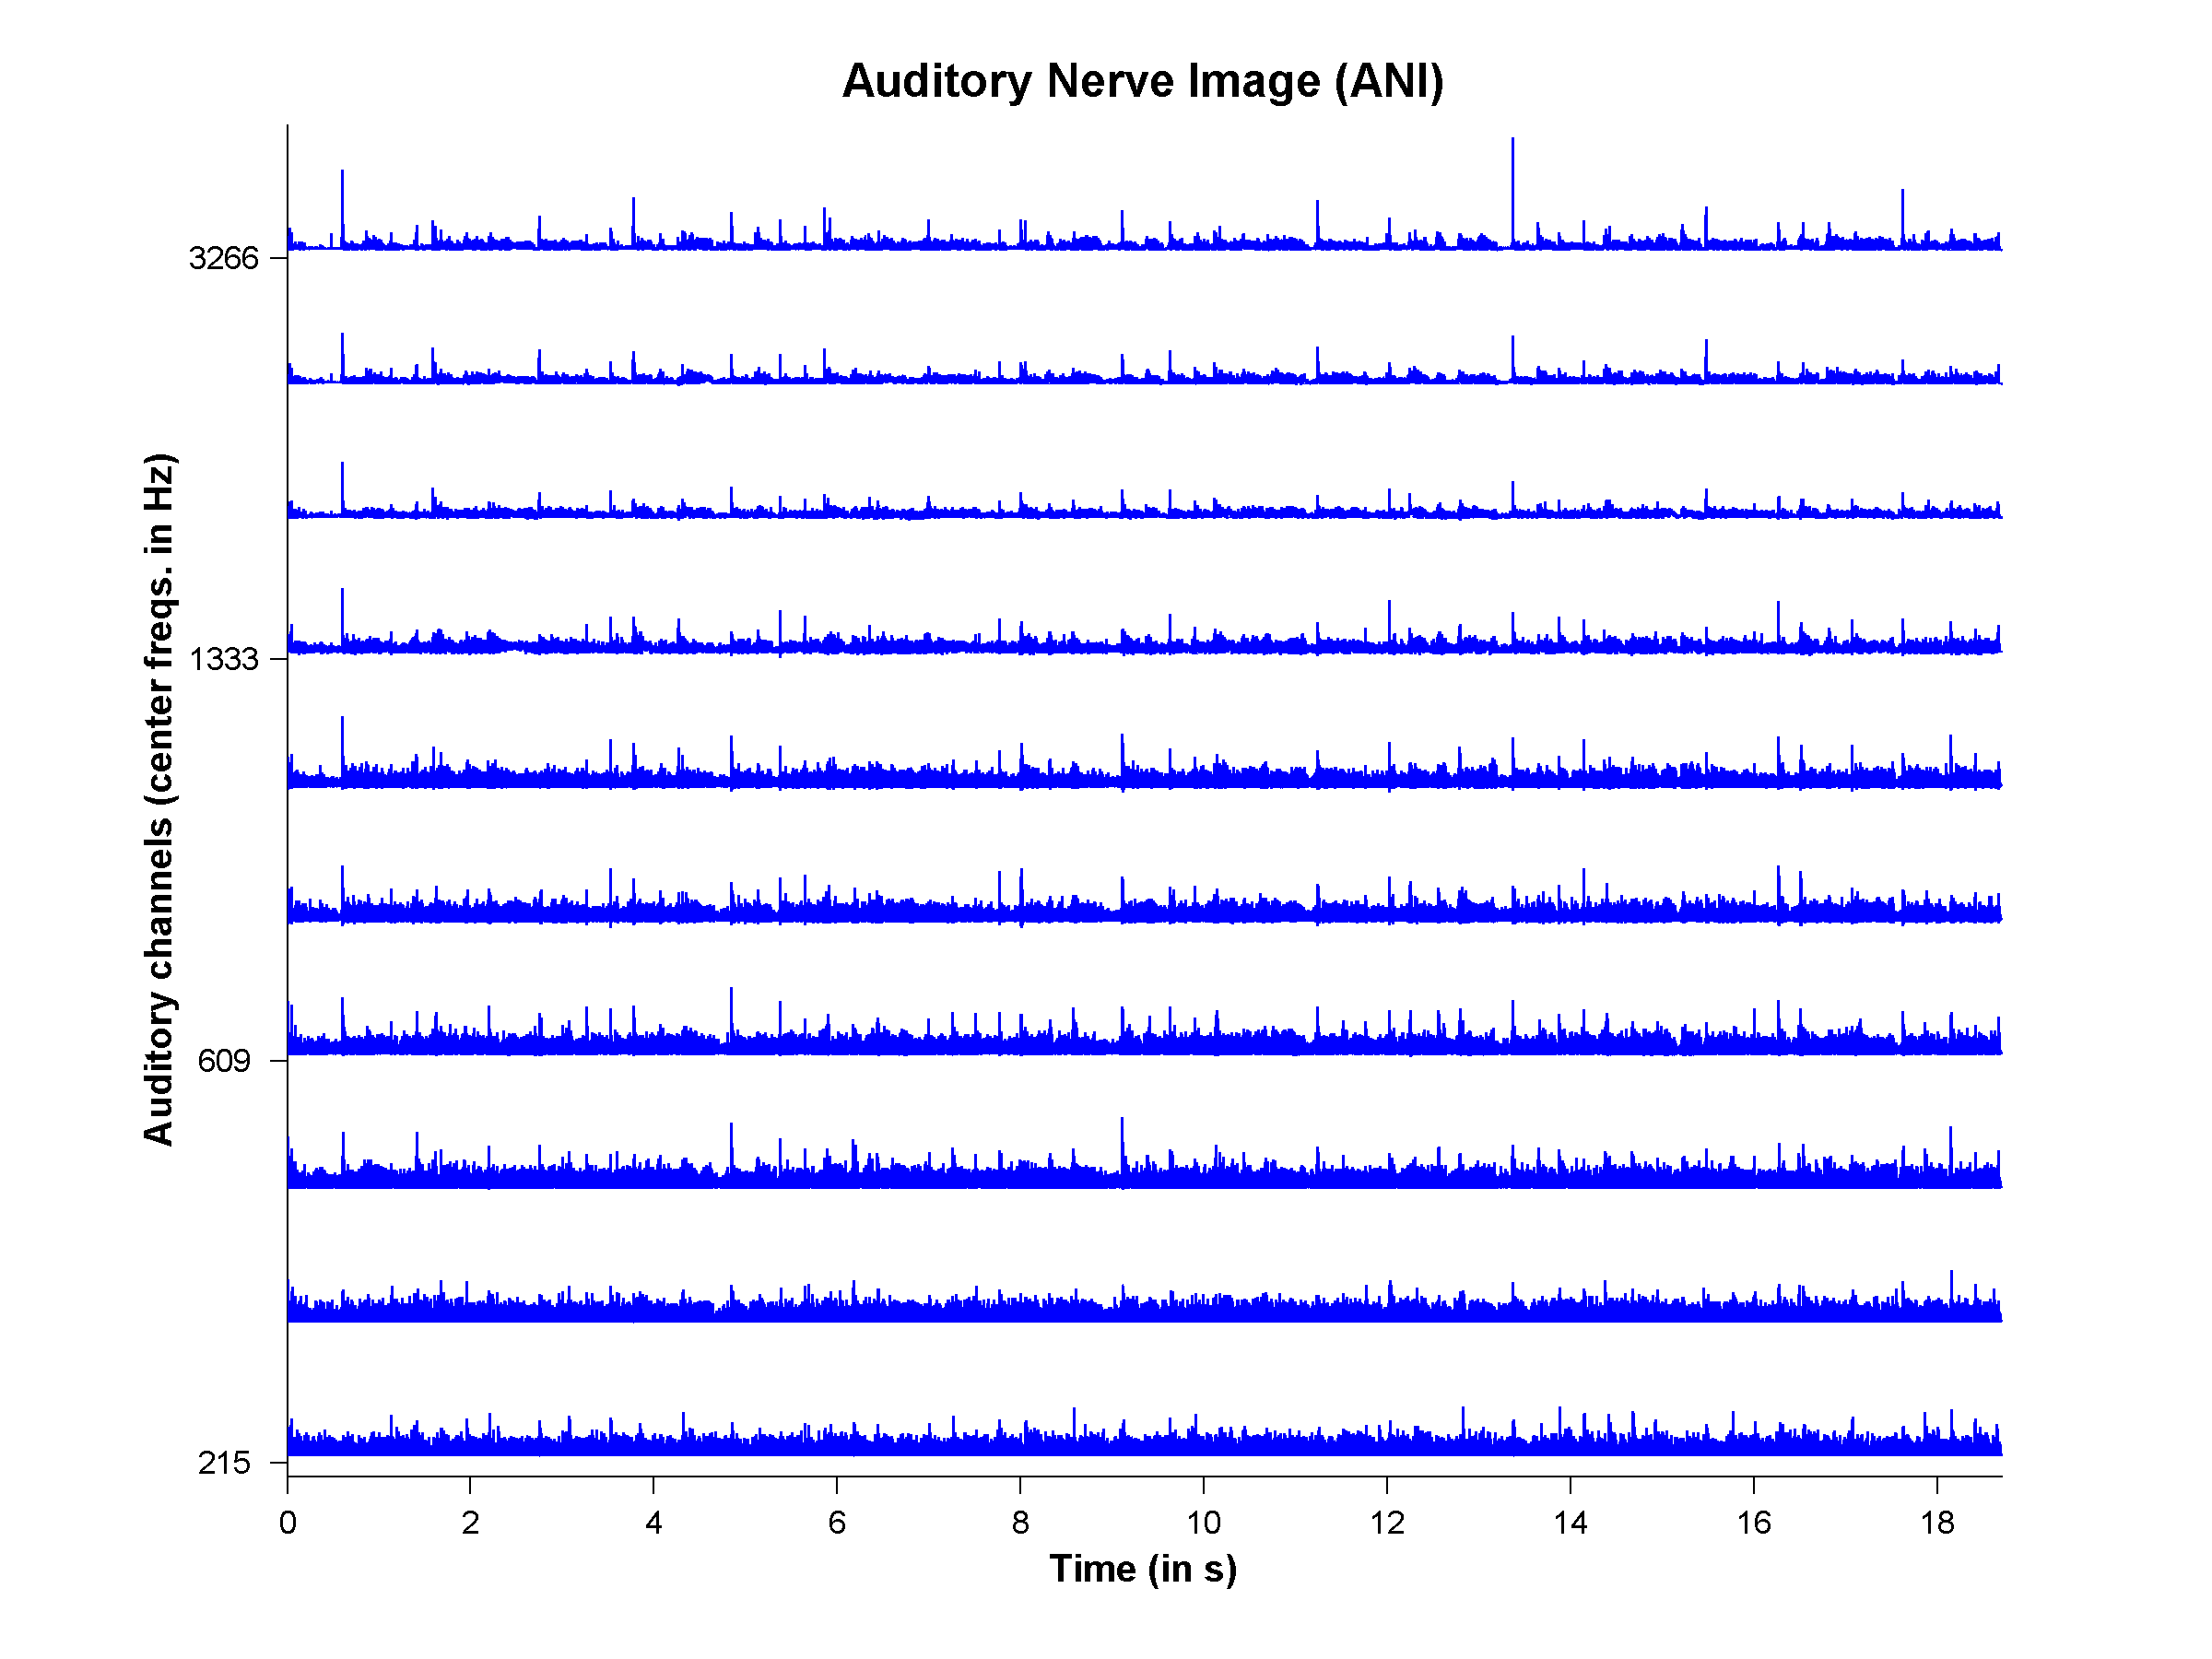
\includegraphics[width=7.5cm]{Graphics/MECDemoTomWaitsBigInJapanANI} & 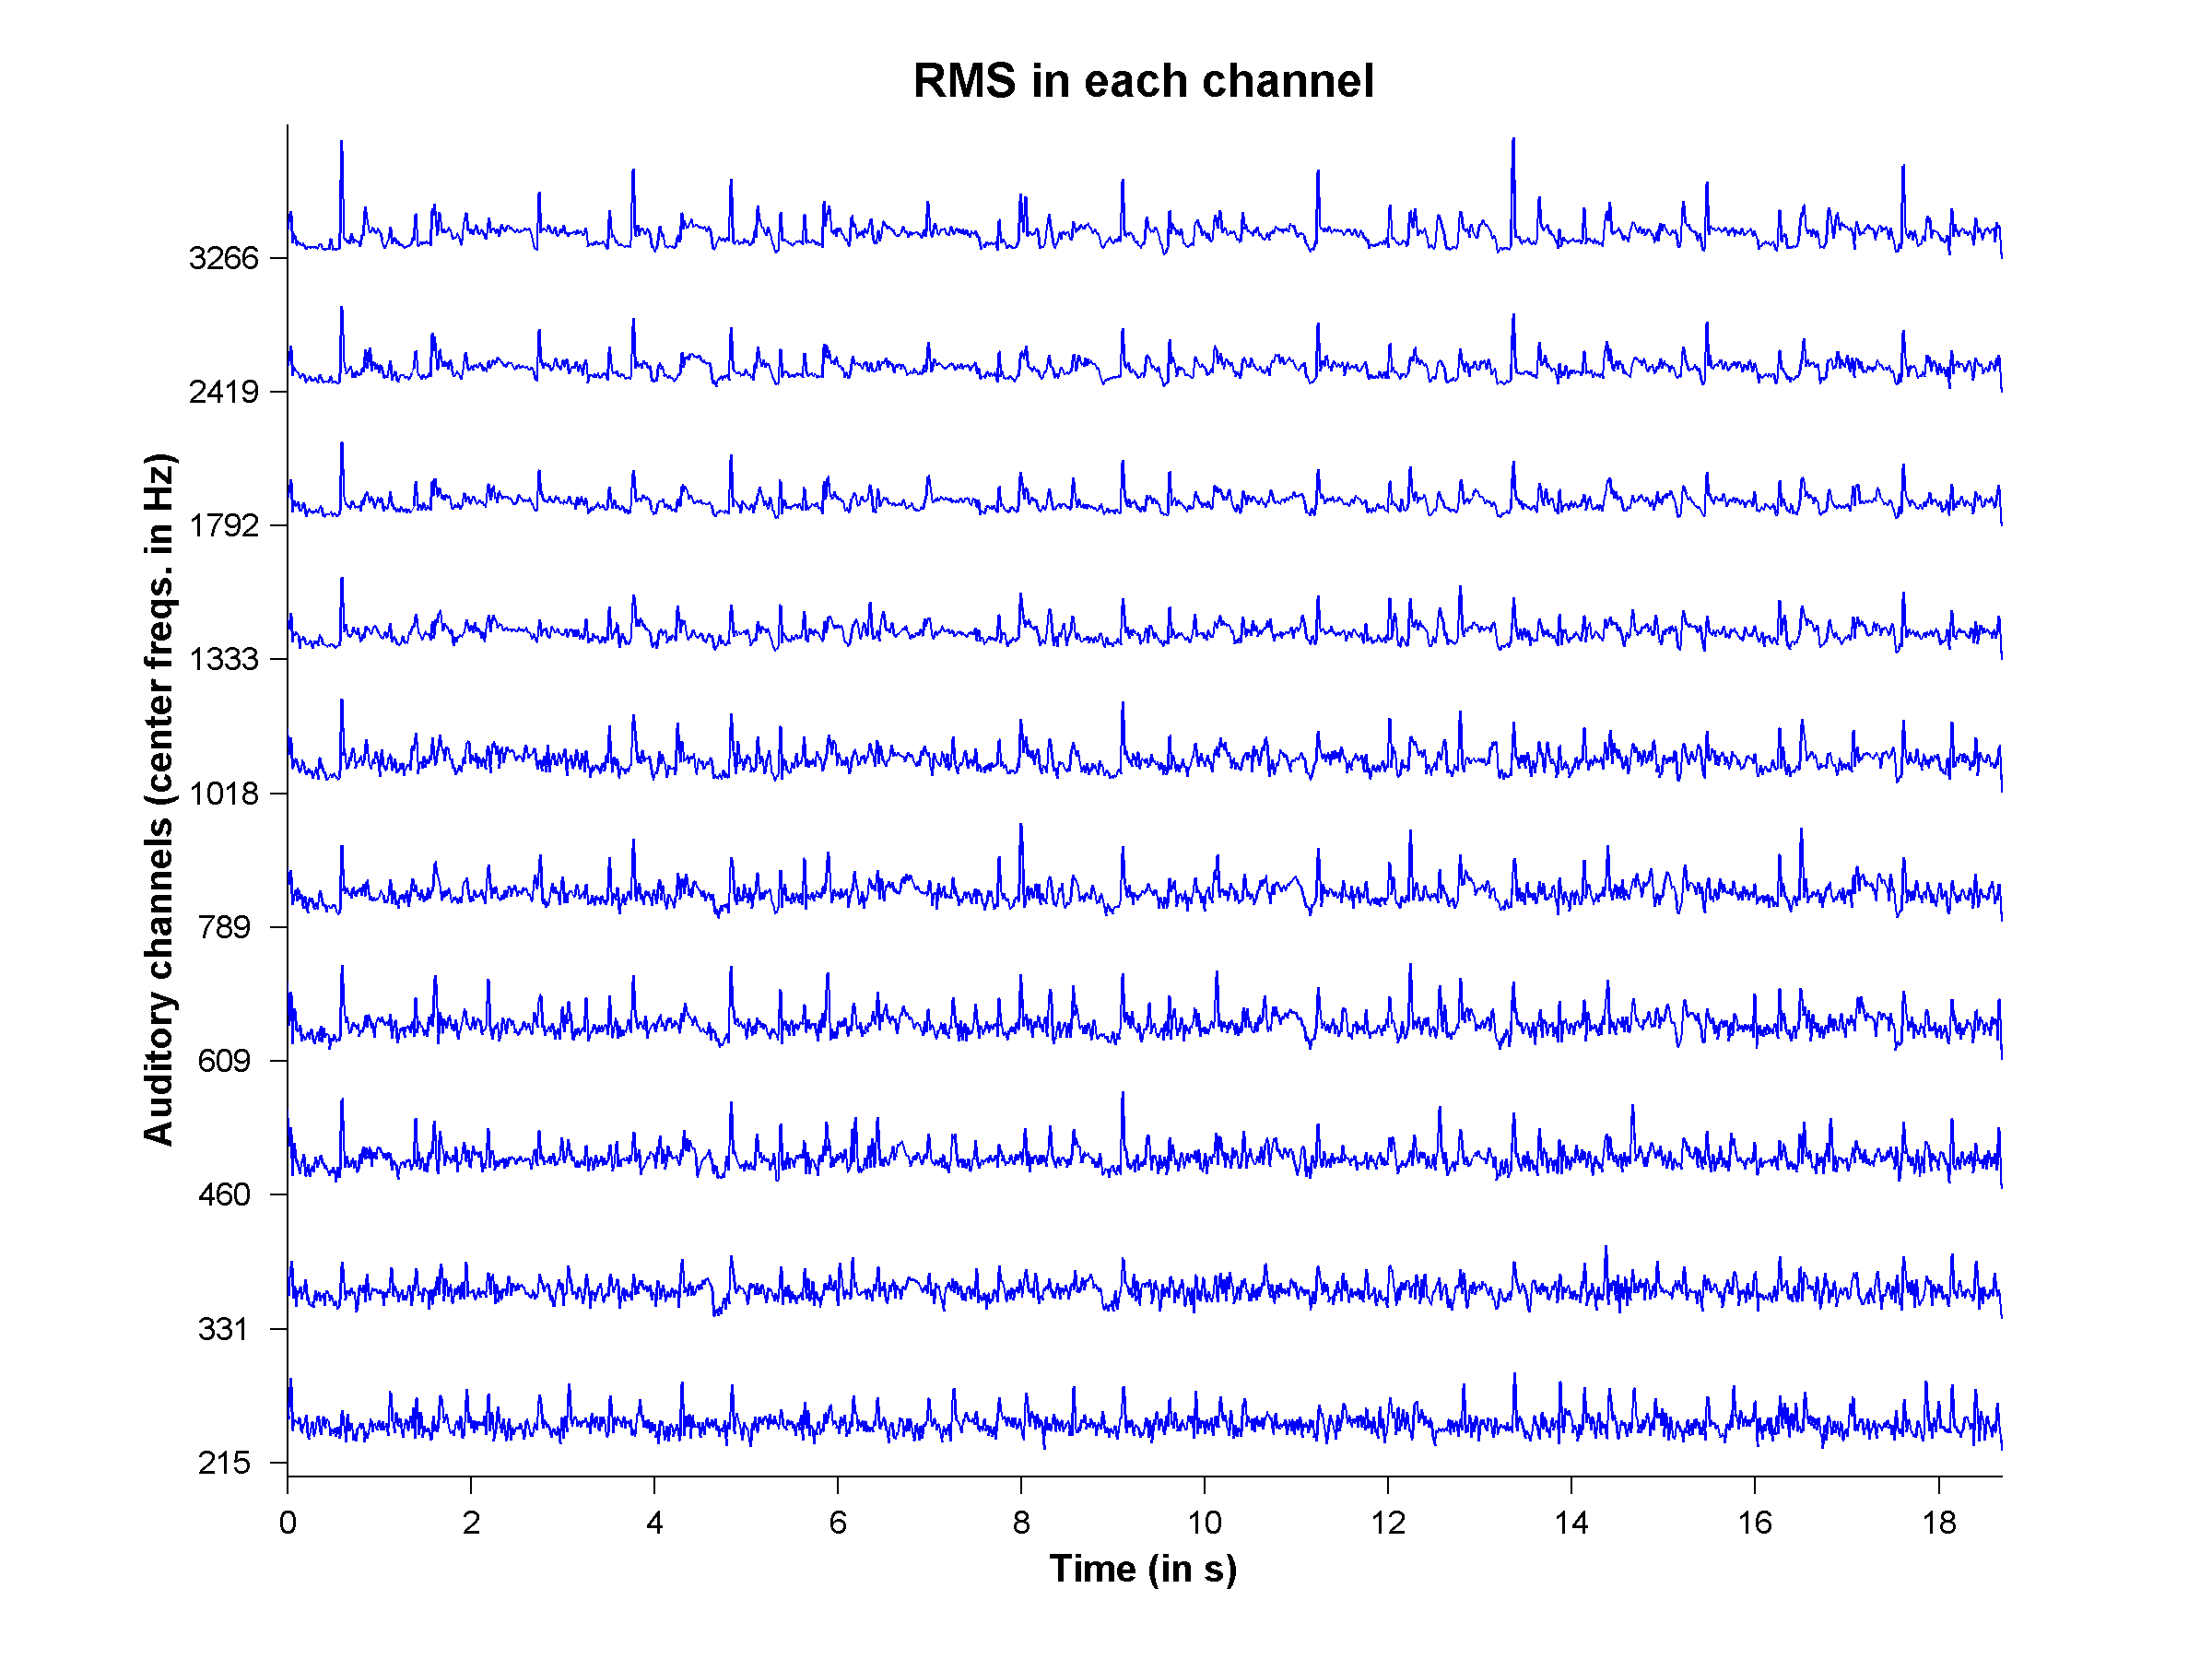
\includegraphics[width=7.5cm]{Graphics/MECDemoTomWaitsBigInJapanANIRMS}\\
        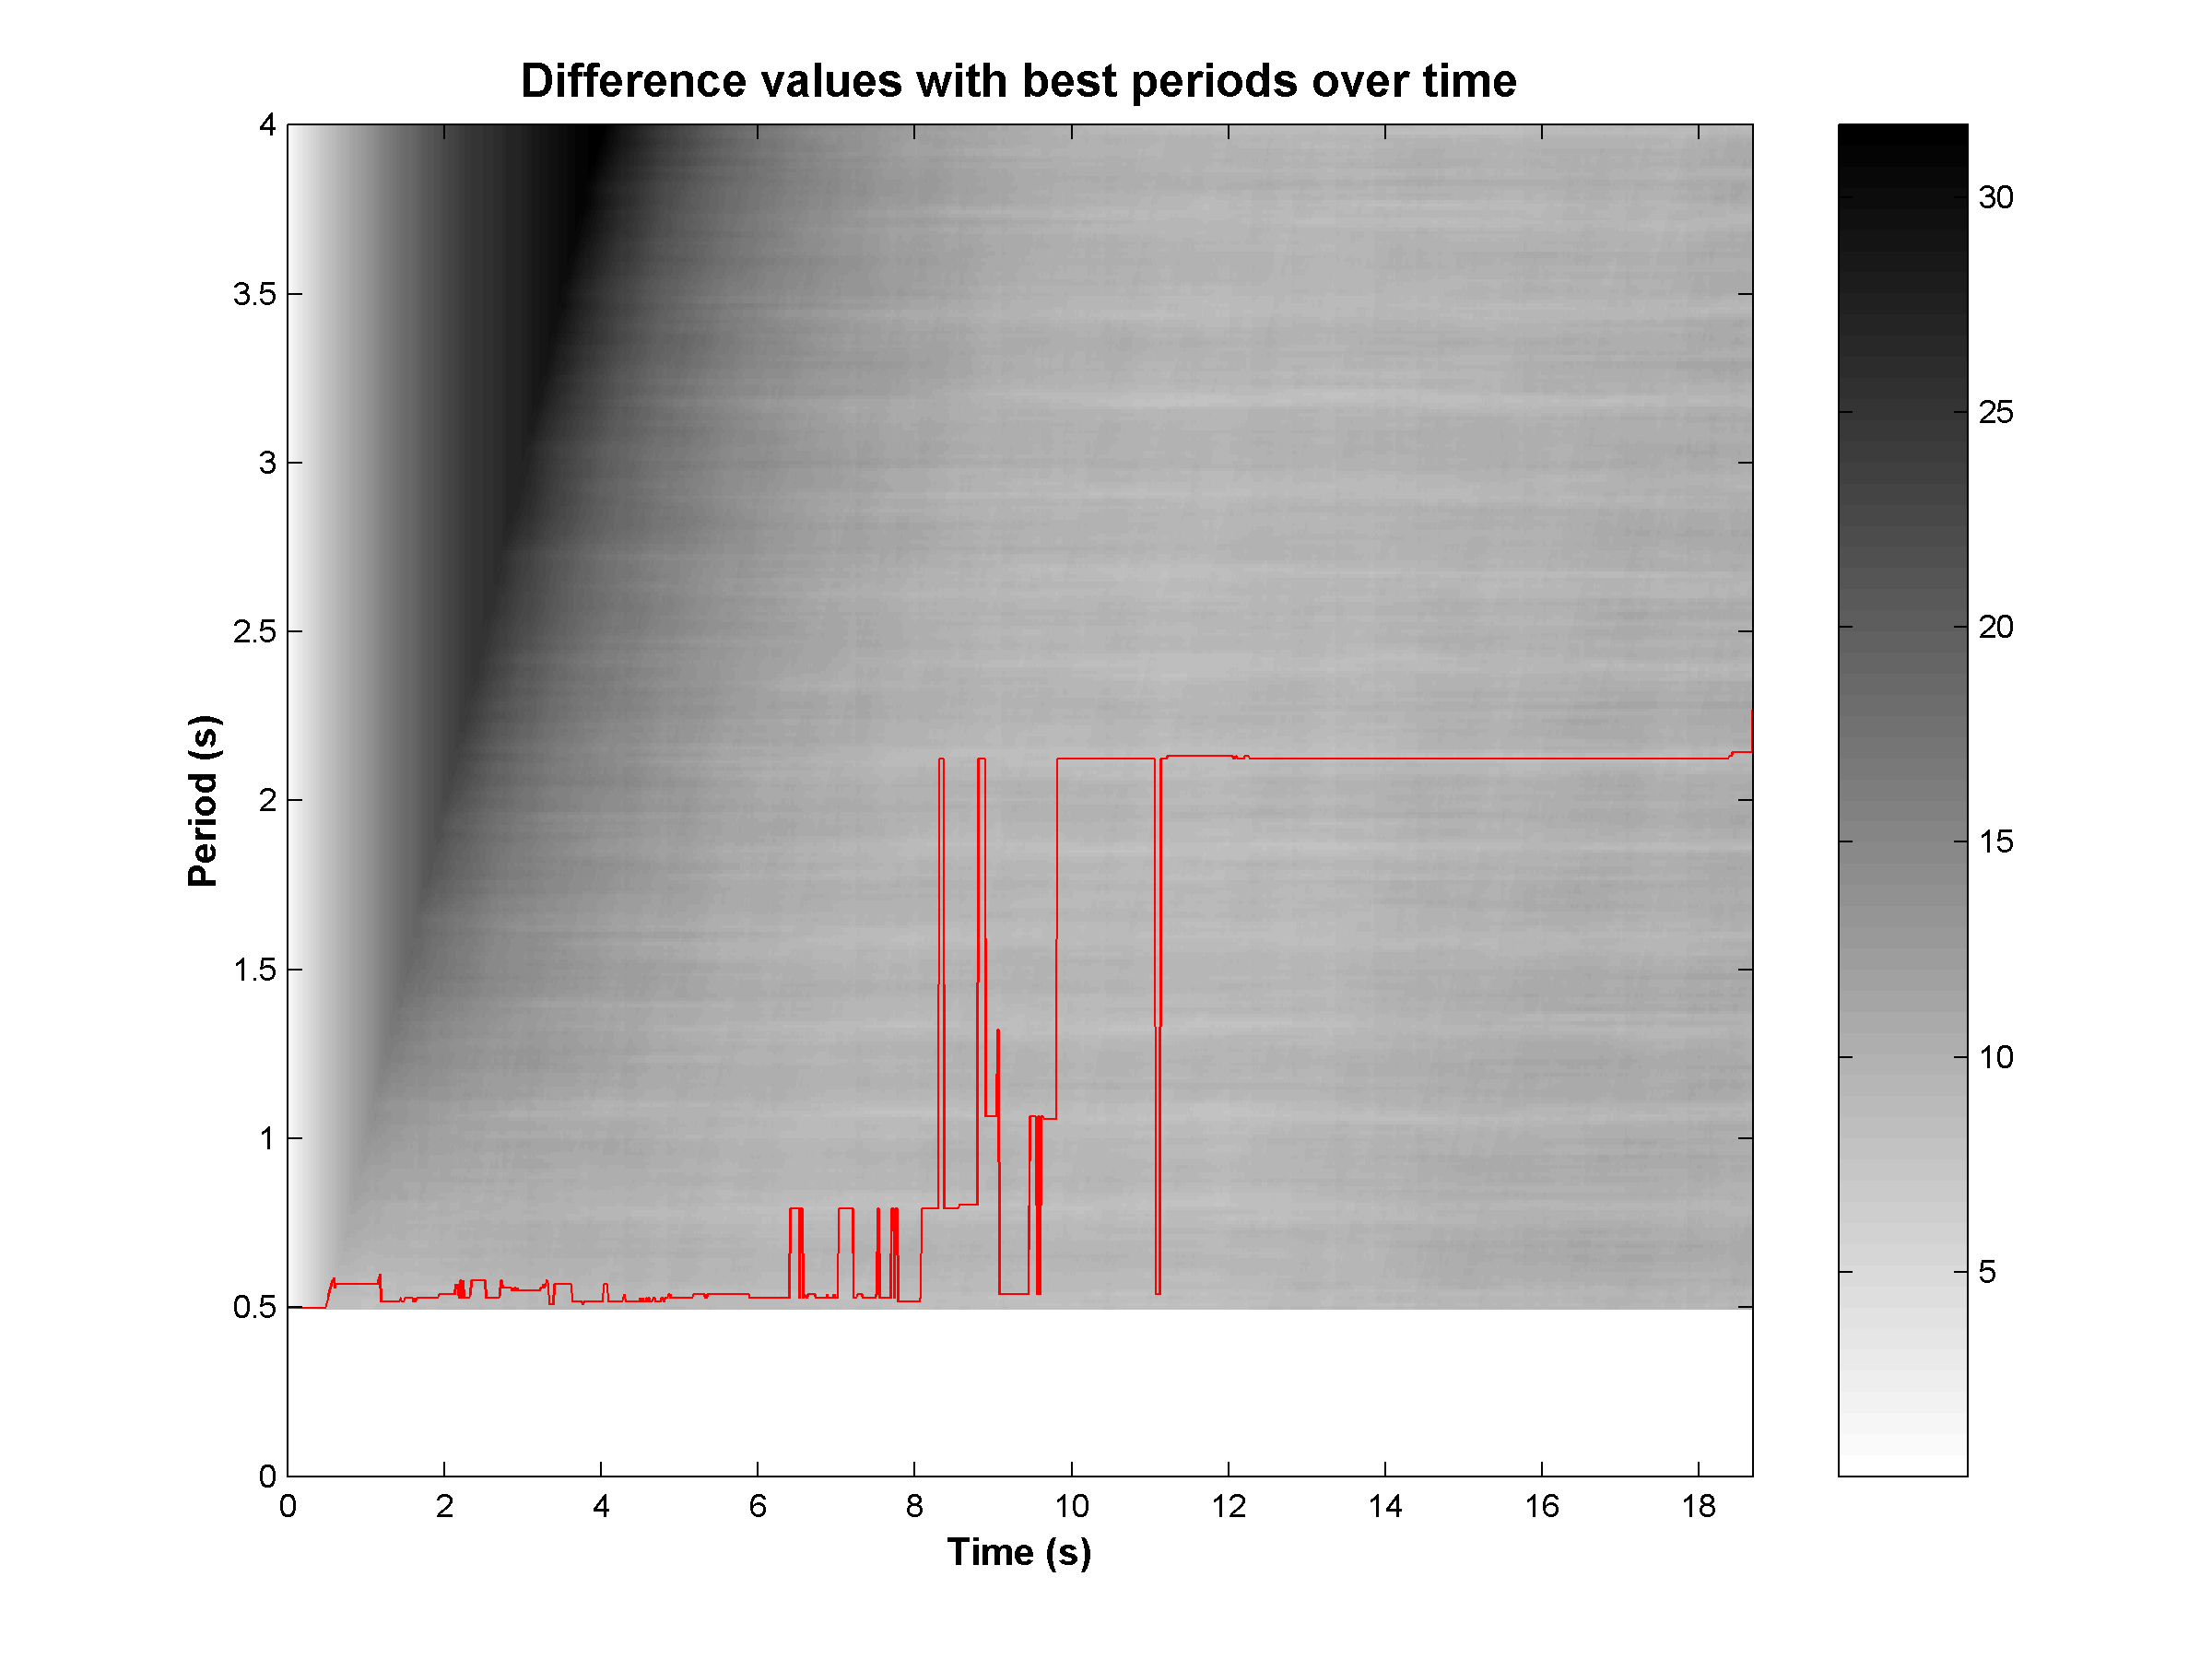
\includegraphics[width=7.5cm]{Graphics/MECDemoTomWaitsBigInJapanValues} & 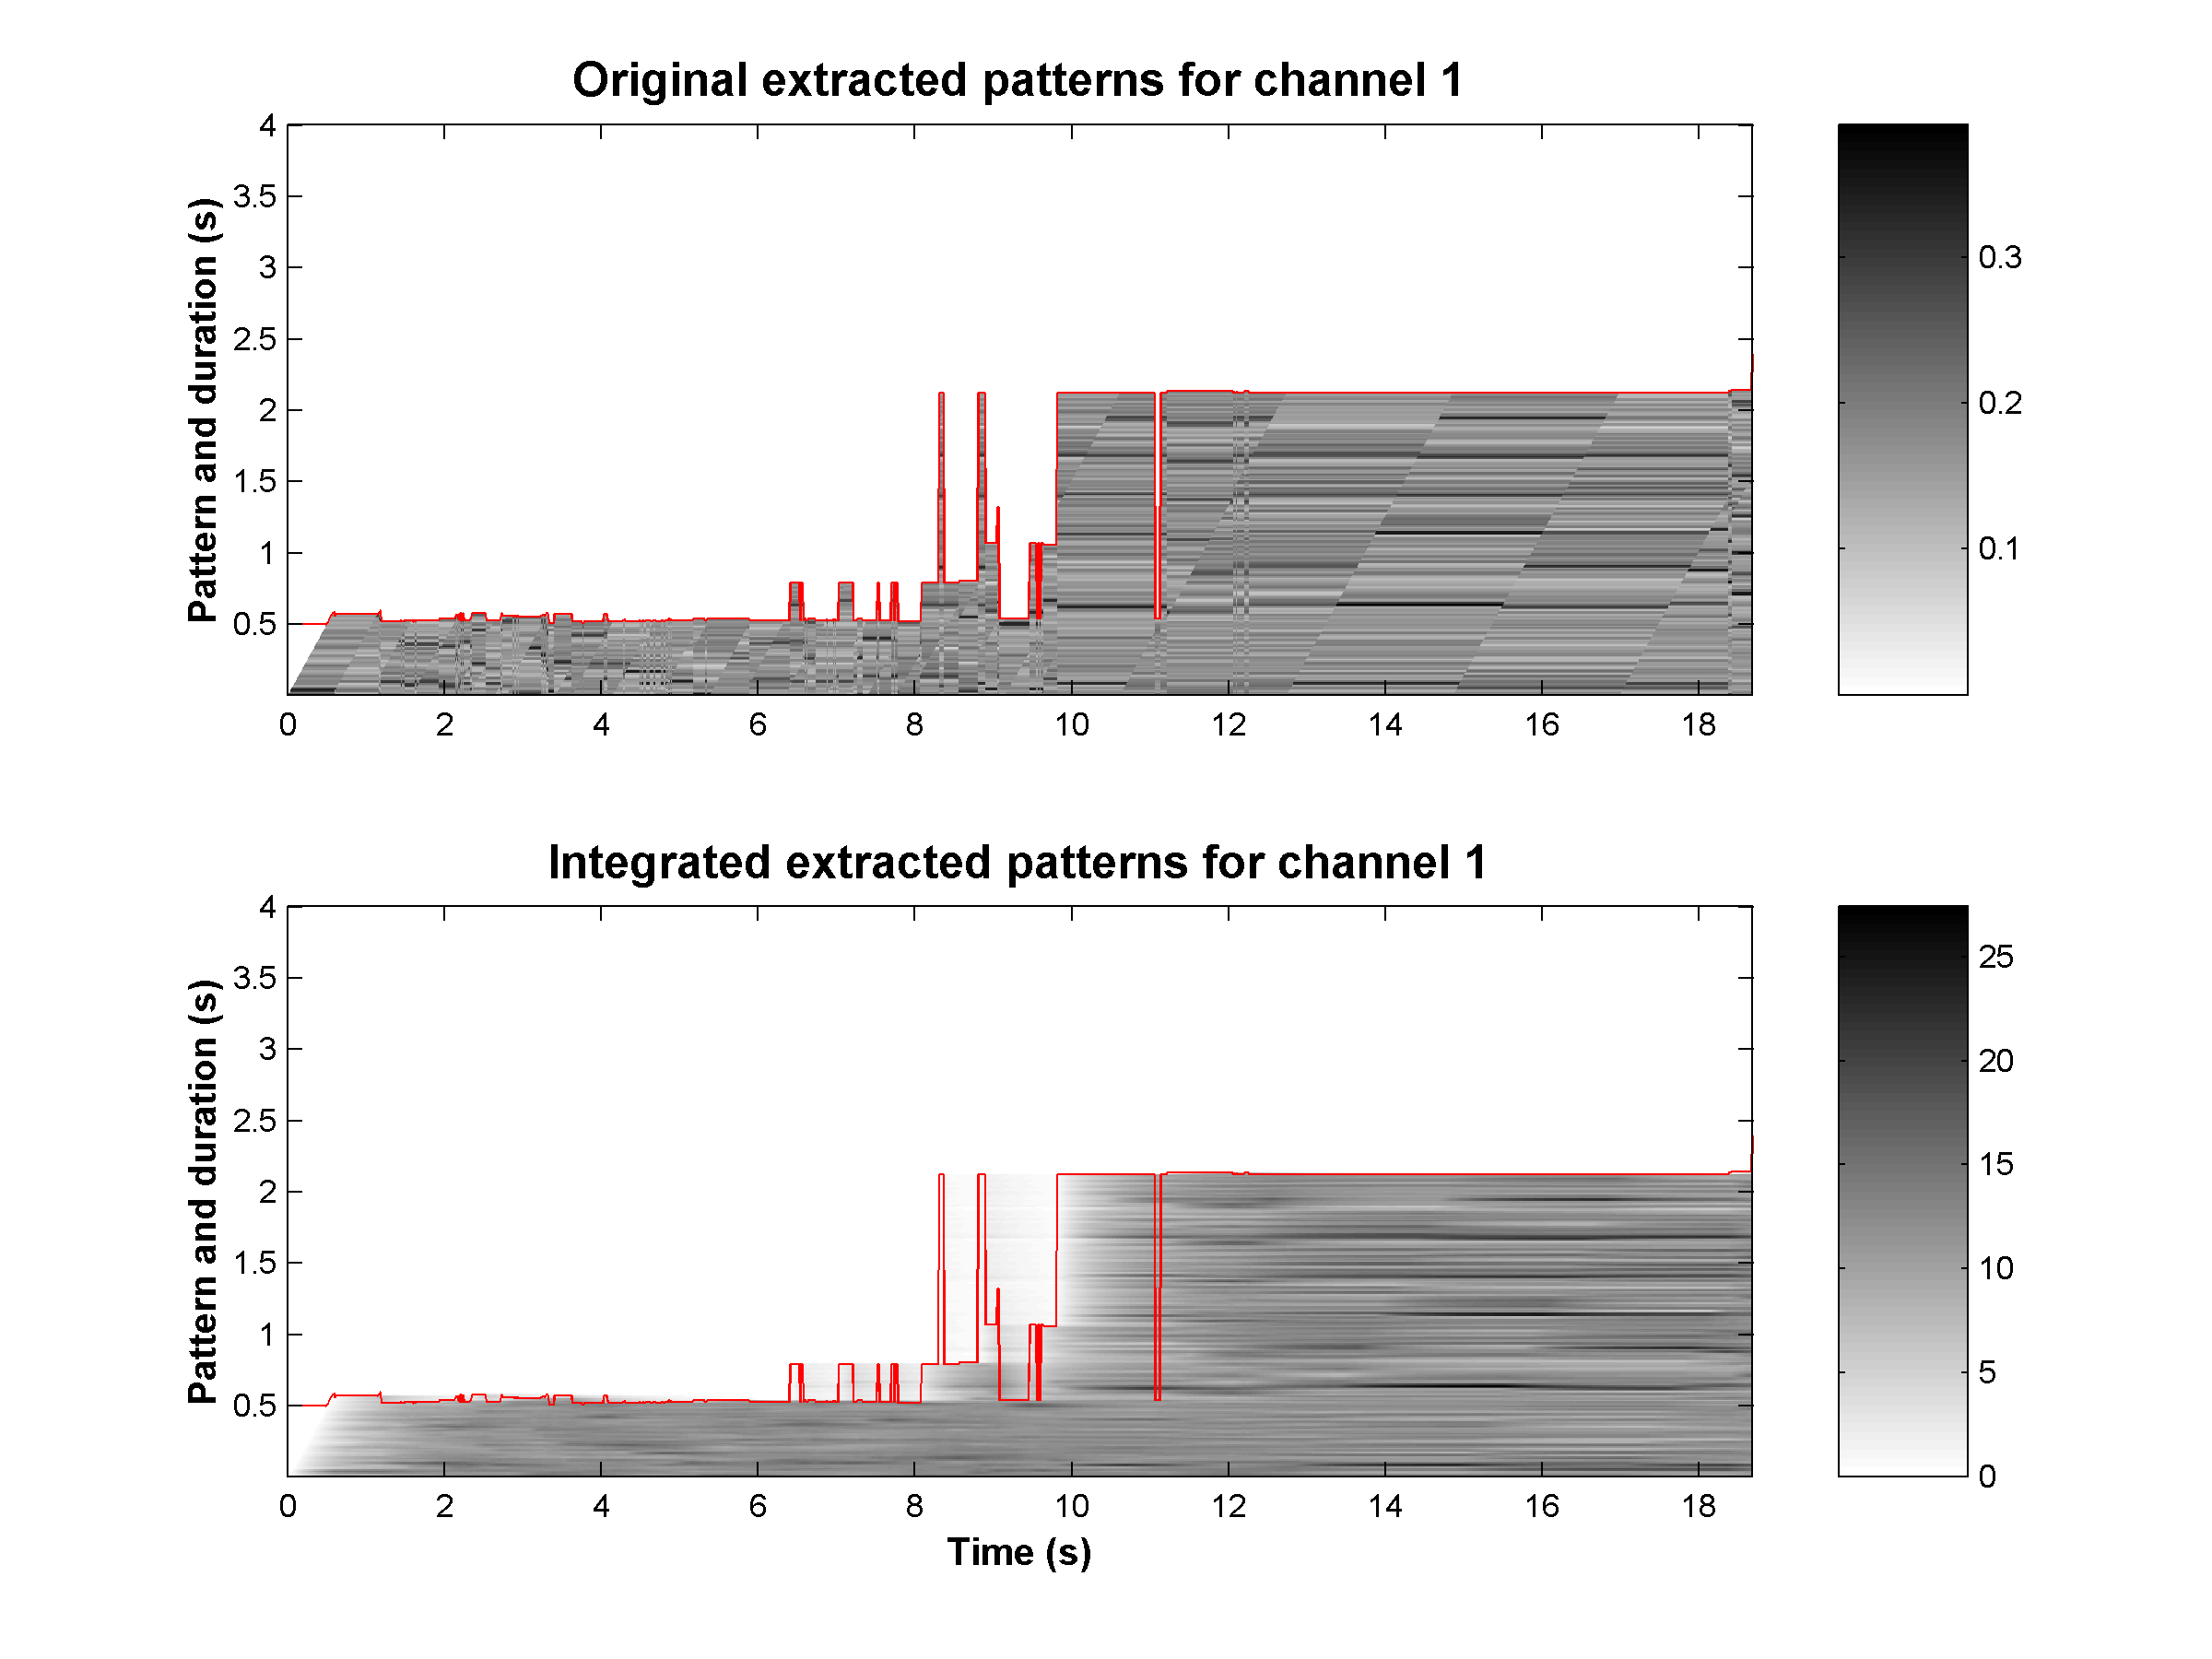
\includegraphics[width=7.5cm]{Graphics/MECDemoTomWaitsBigInJapanIntegrPattCh1}\\
        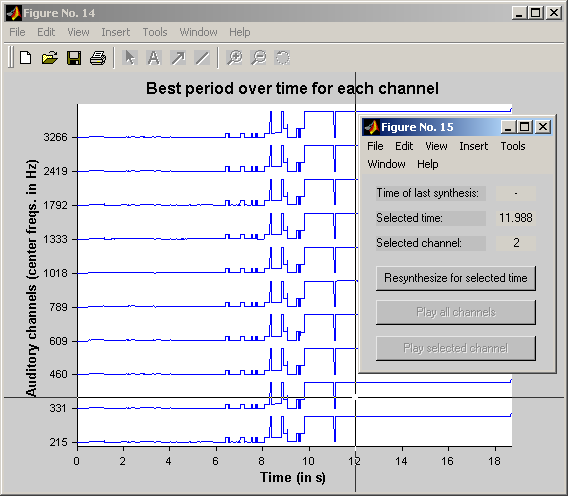
\includegraphics[width=7.5cm]{Graphics/MECDemoTomWaitsBigInJapanUI} & \\
    \end{tabular}
    \caption{Results for TomWaitsBigInJapan.wav}
    \label{Fig:MECTomWaitsExample}
\end{figure}

\begin{figure}[p]
    \begin{tabular}{cc}
        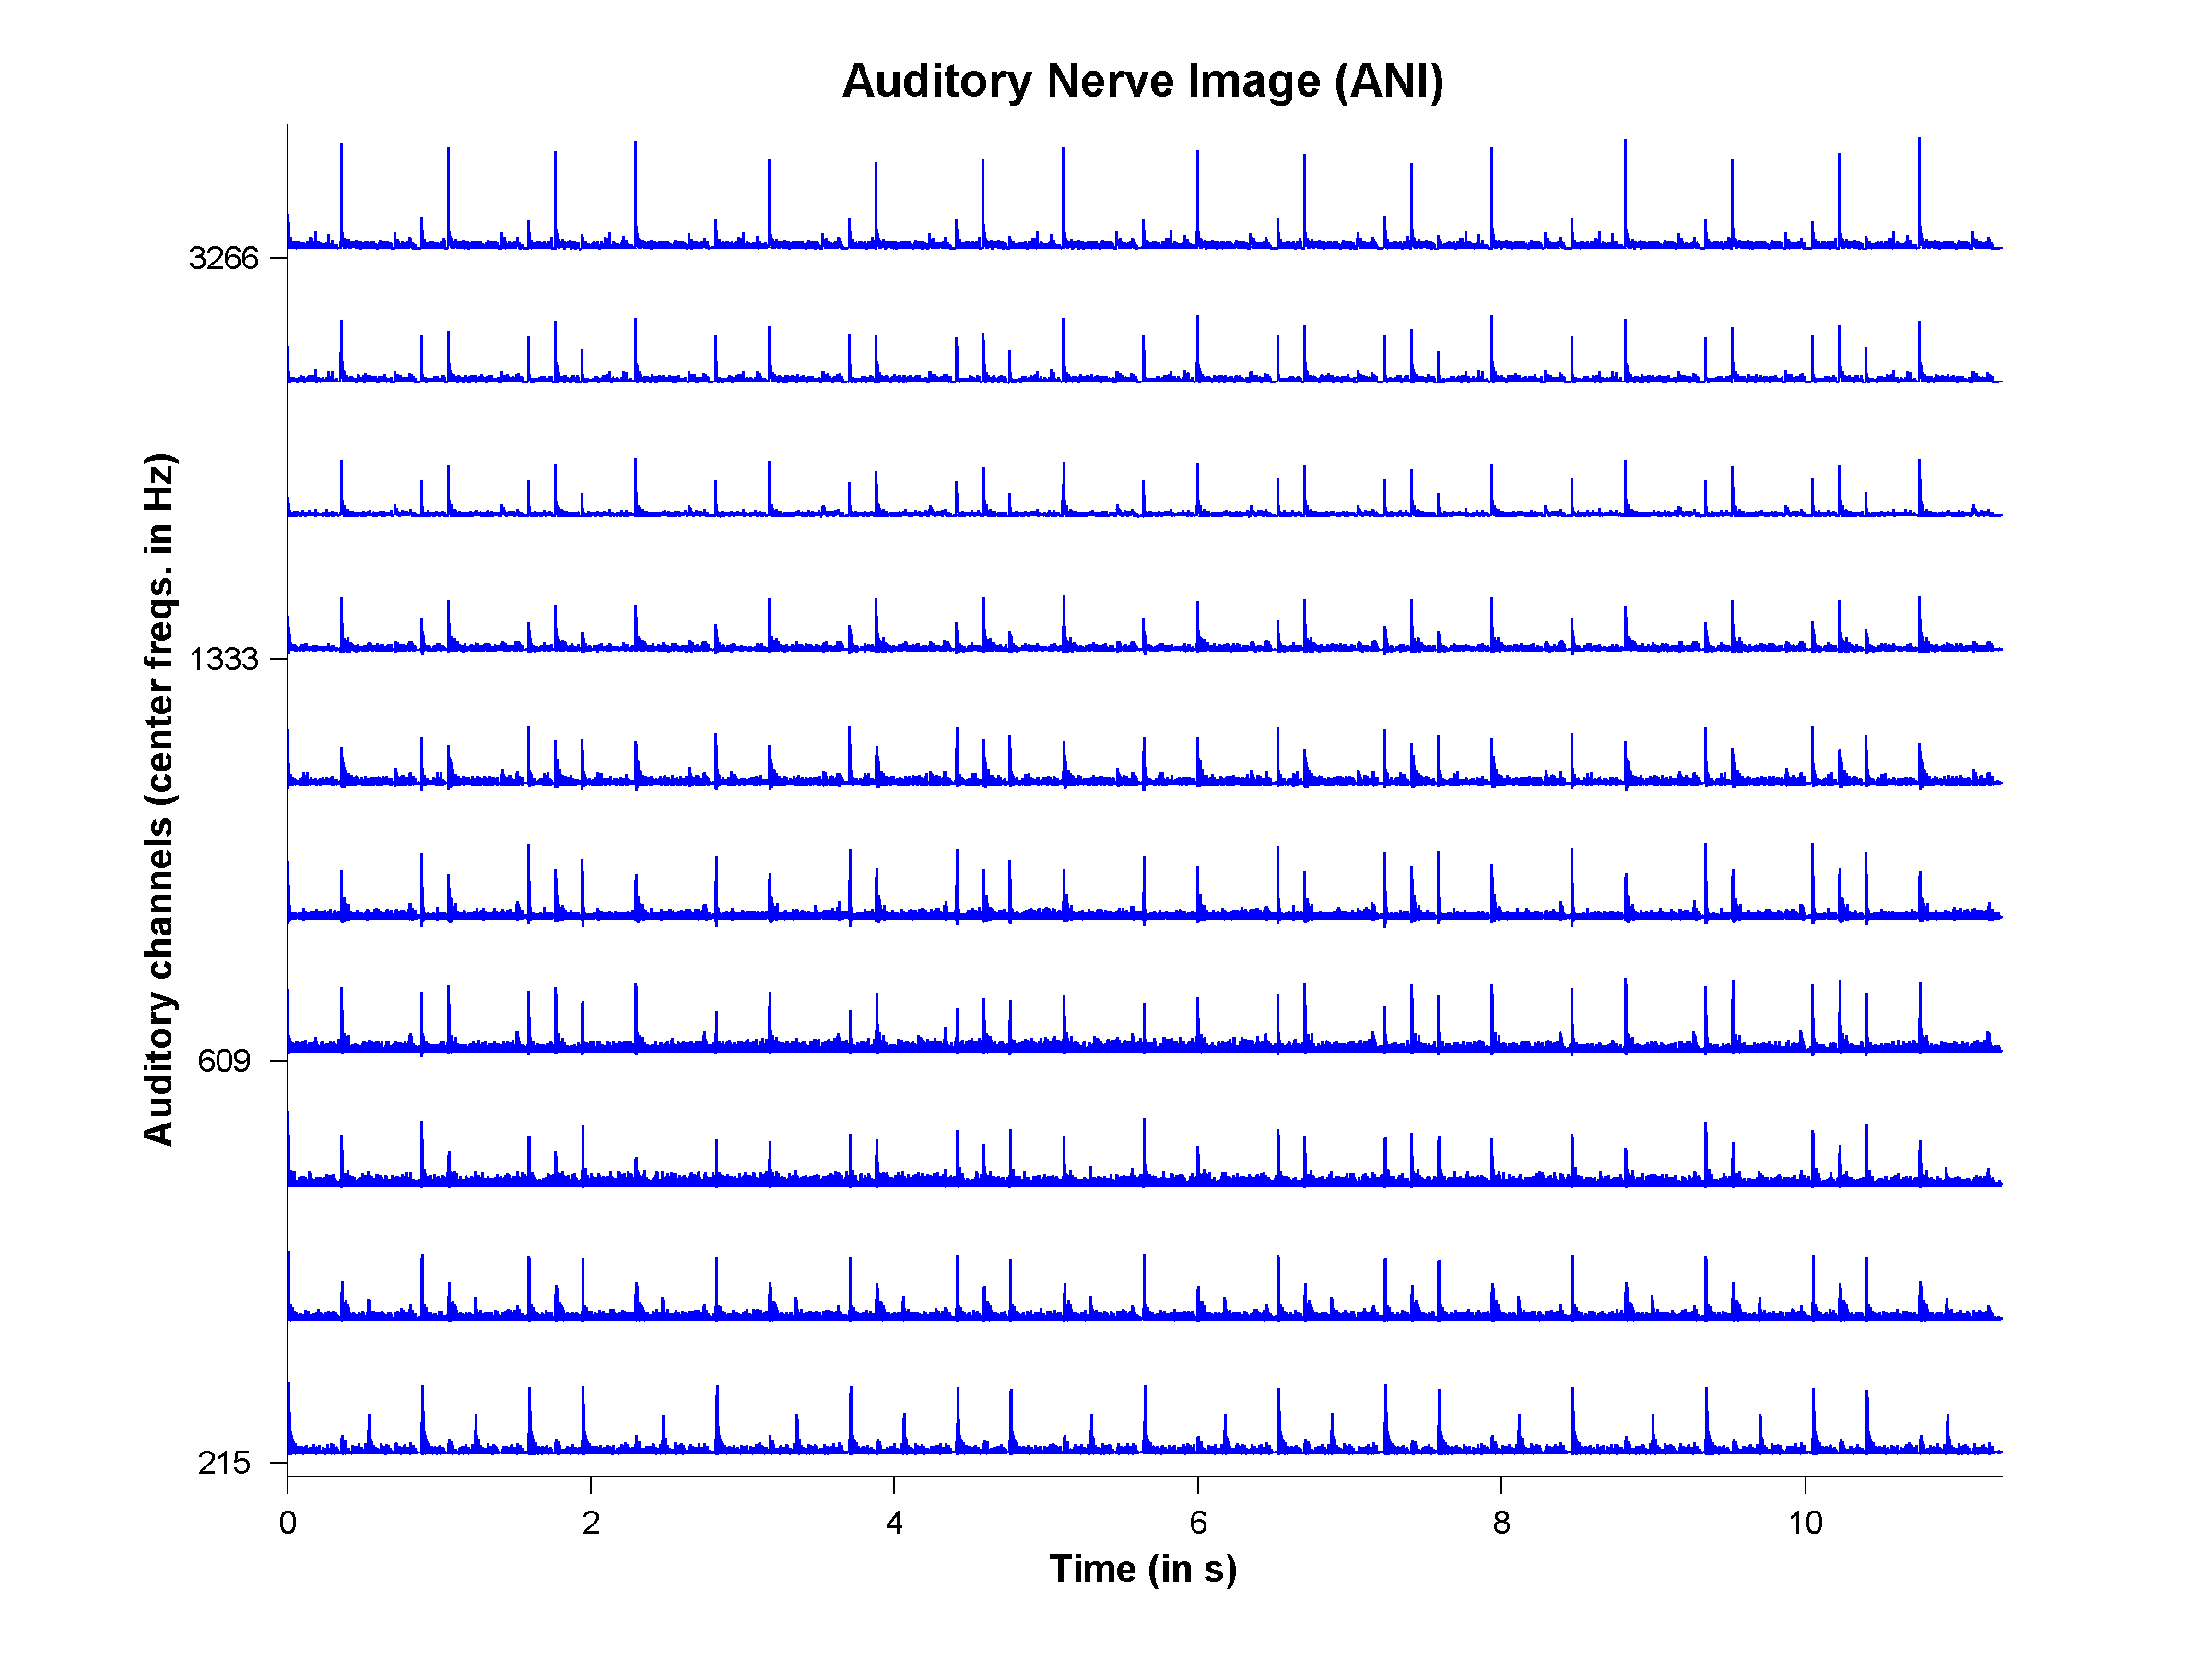
\includegraphics[width=7.5cm]{Graphics/MECDemoPhotekTheLighteningANI} & 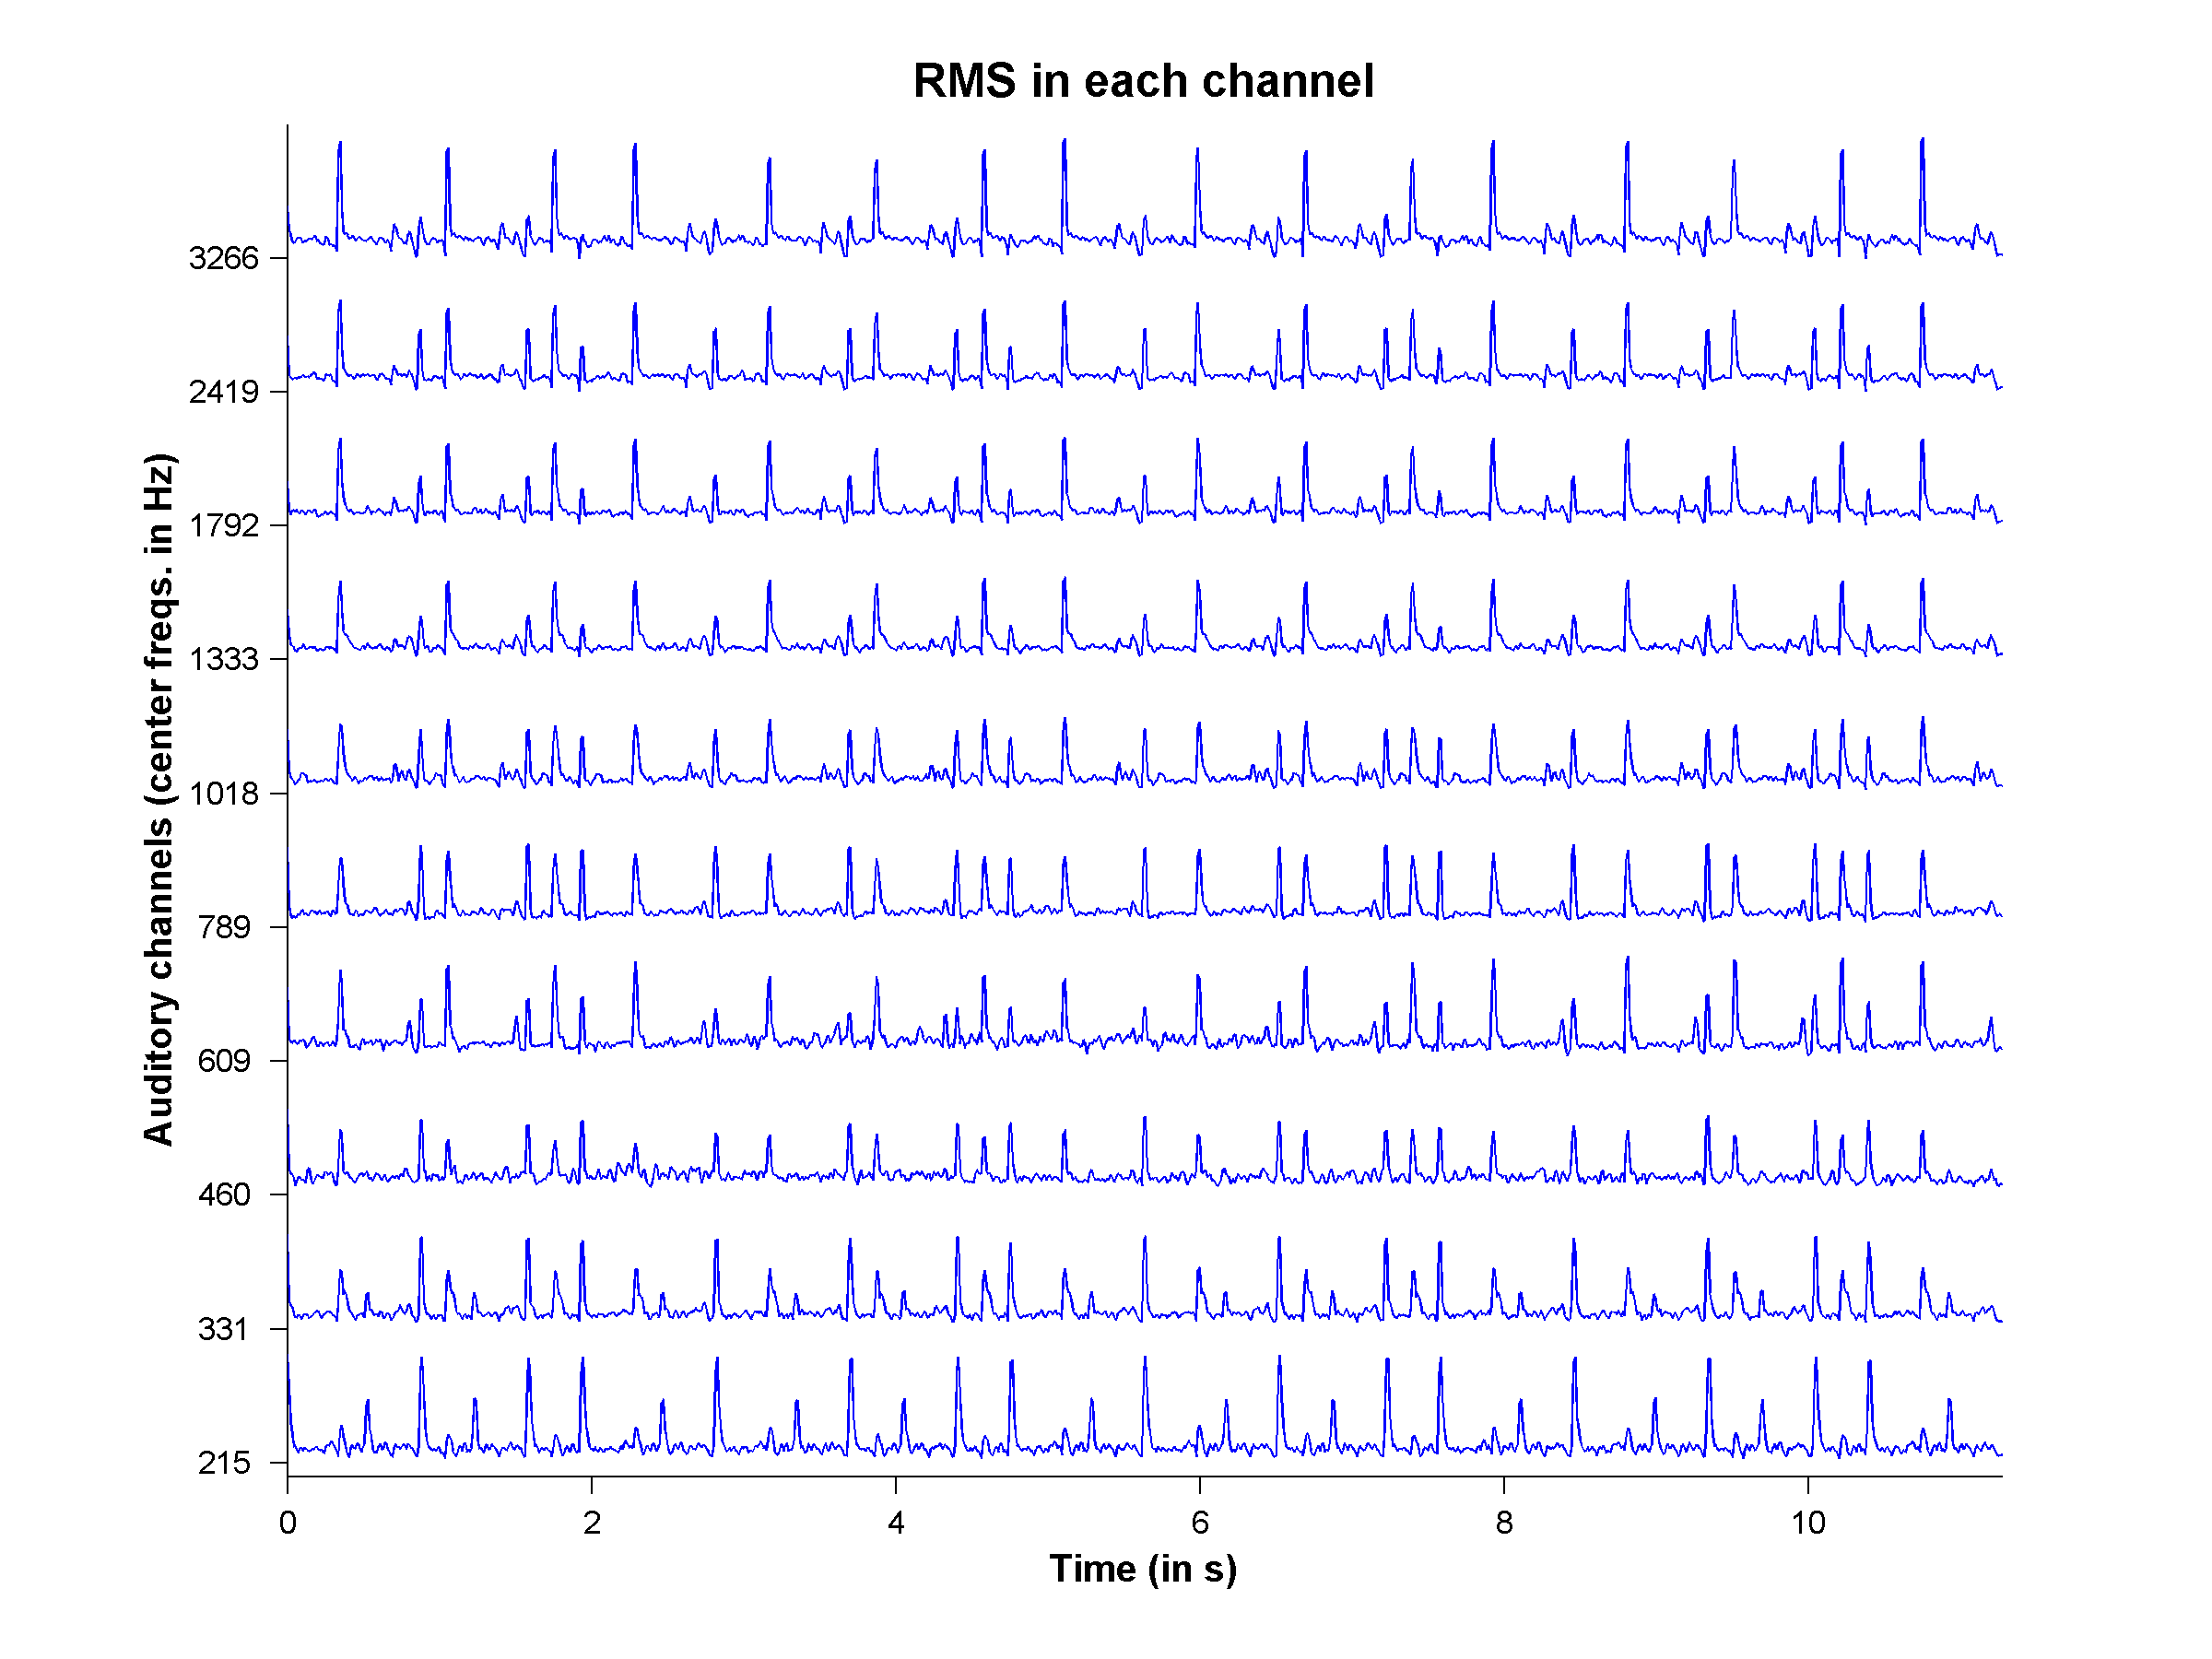
\includegraphics[width=7.5cm]{Graphics/MECDemoPhotekTheLighteningANIRMS}\\
        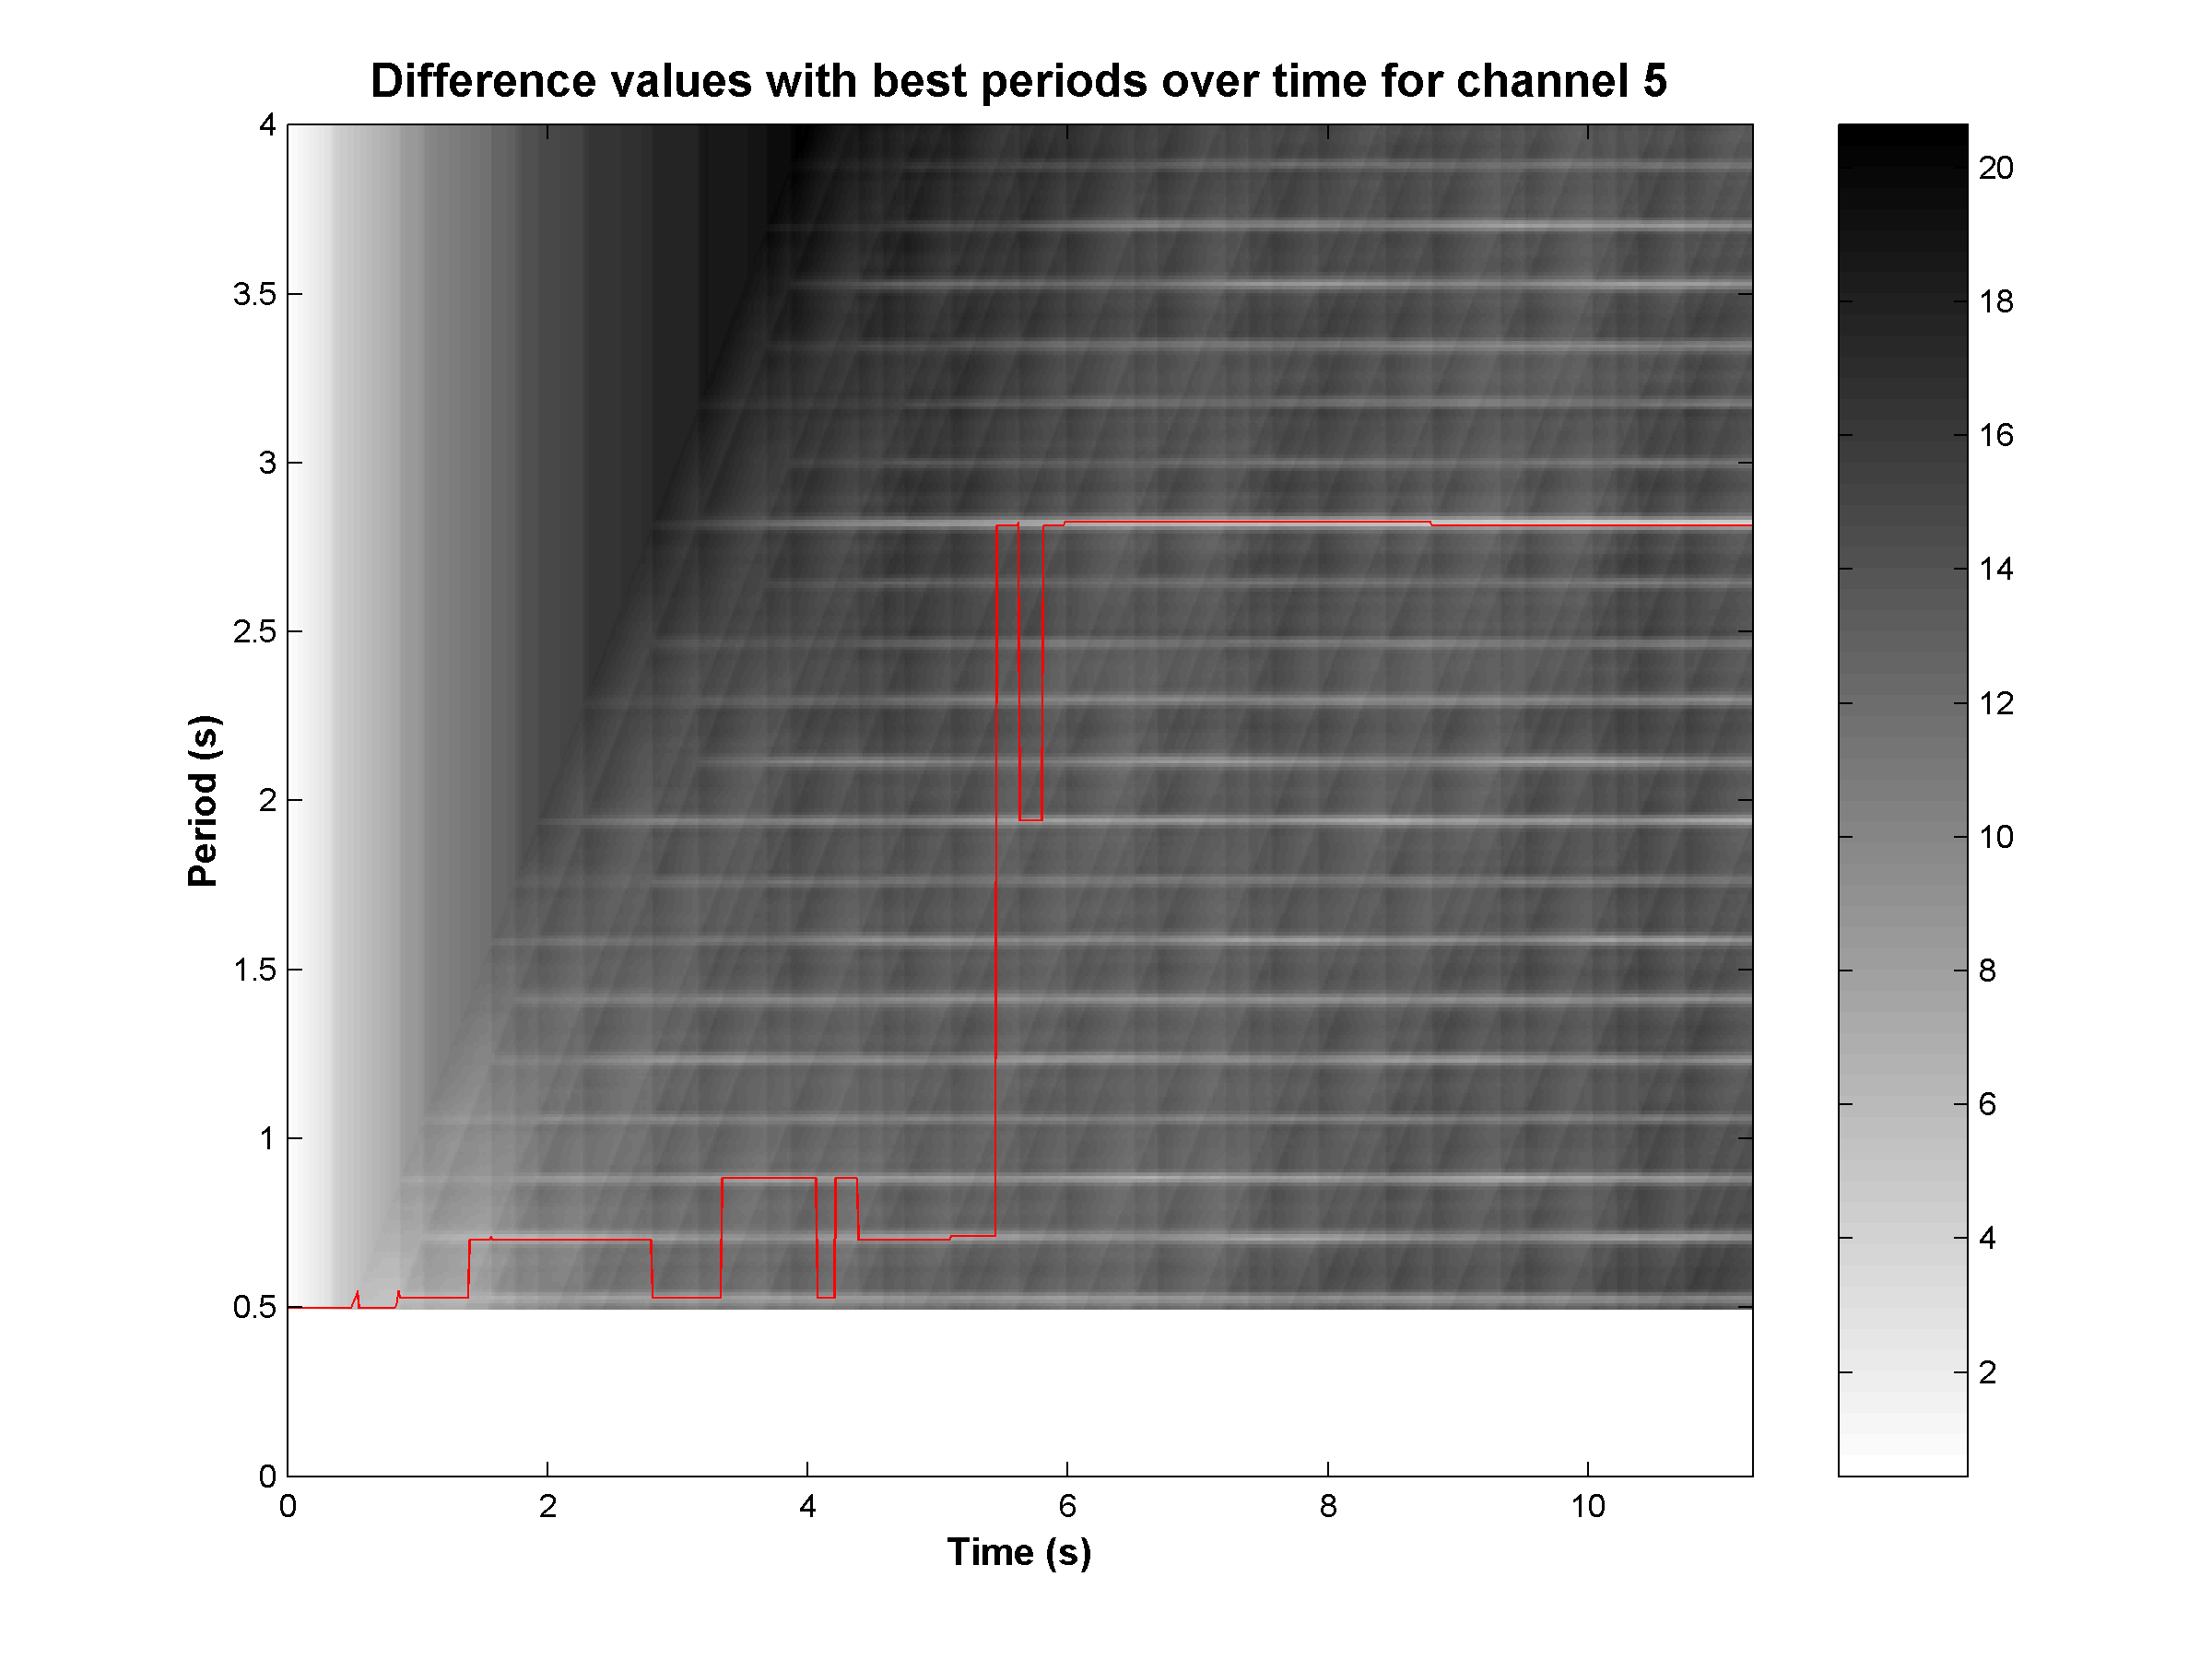
\includegraphics[width=7.5cm]{Graphics/MECDemoPhotekTheLighteningValuesCh5} & 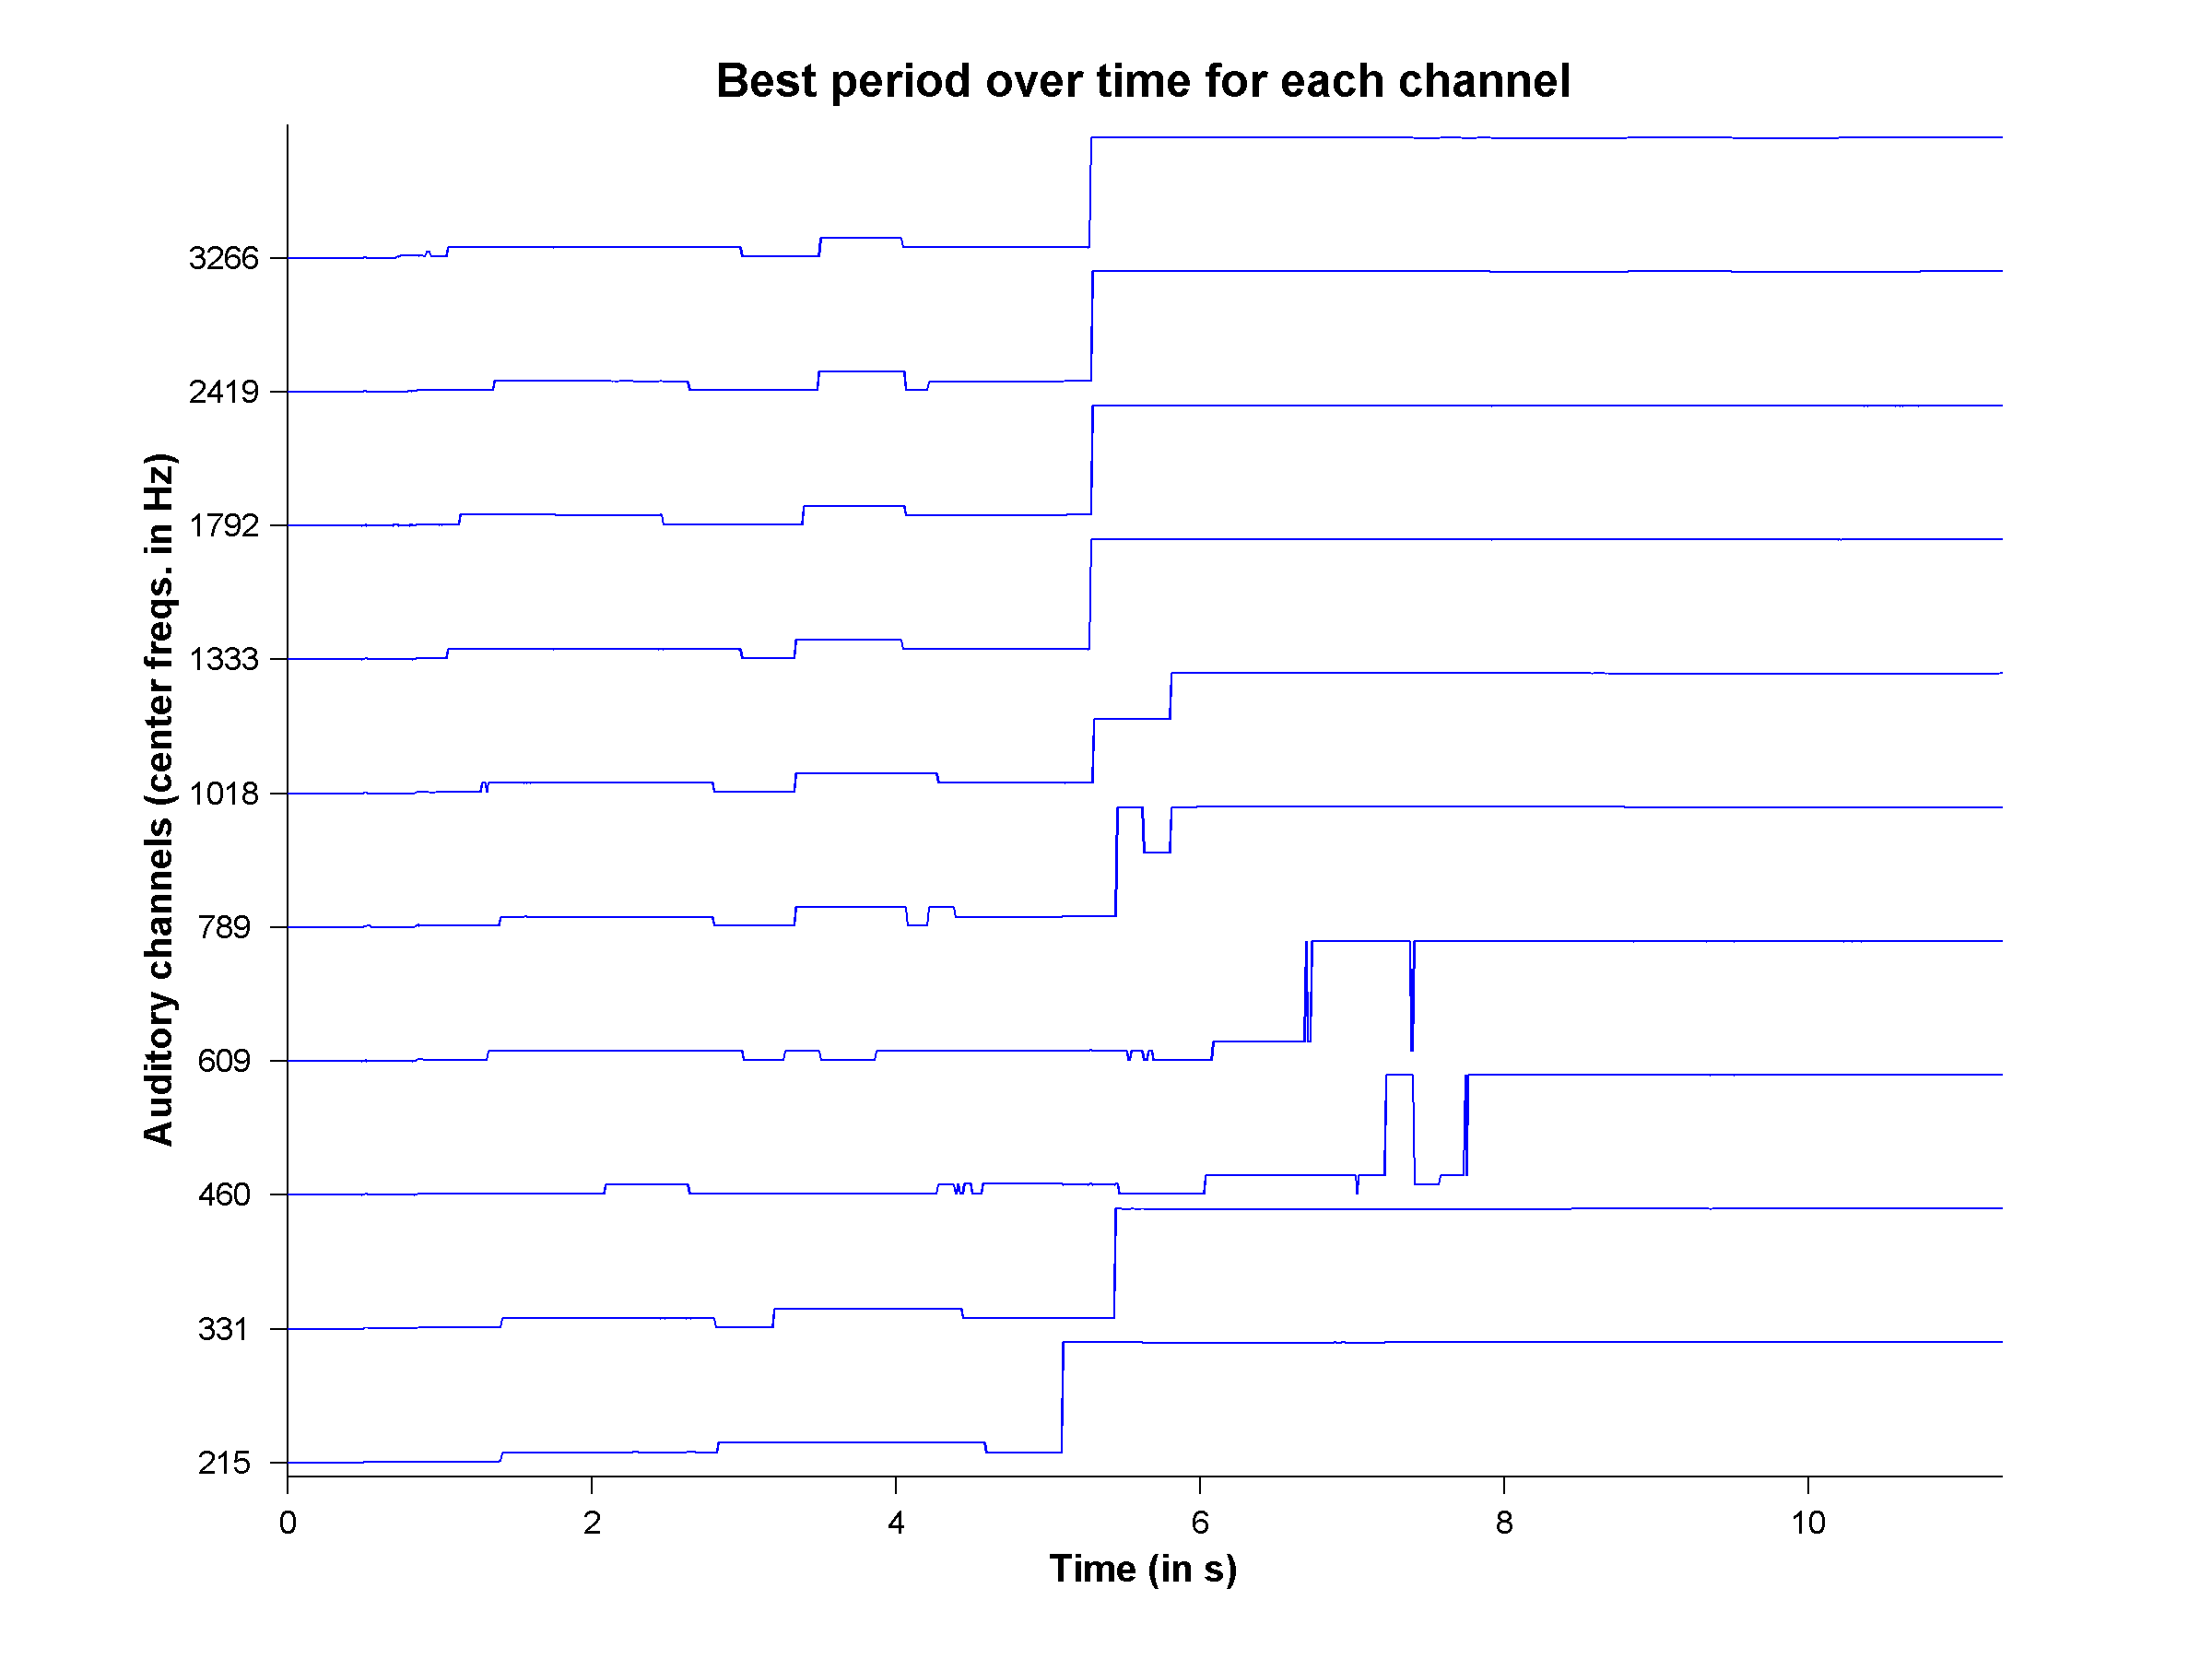
\includegraphics[width=7.5cm]{Graphics/MECDemoPhotekTheLighteningBestPeriodsANI}\\
        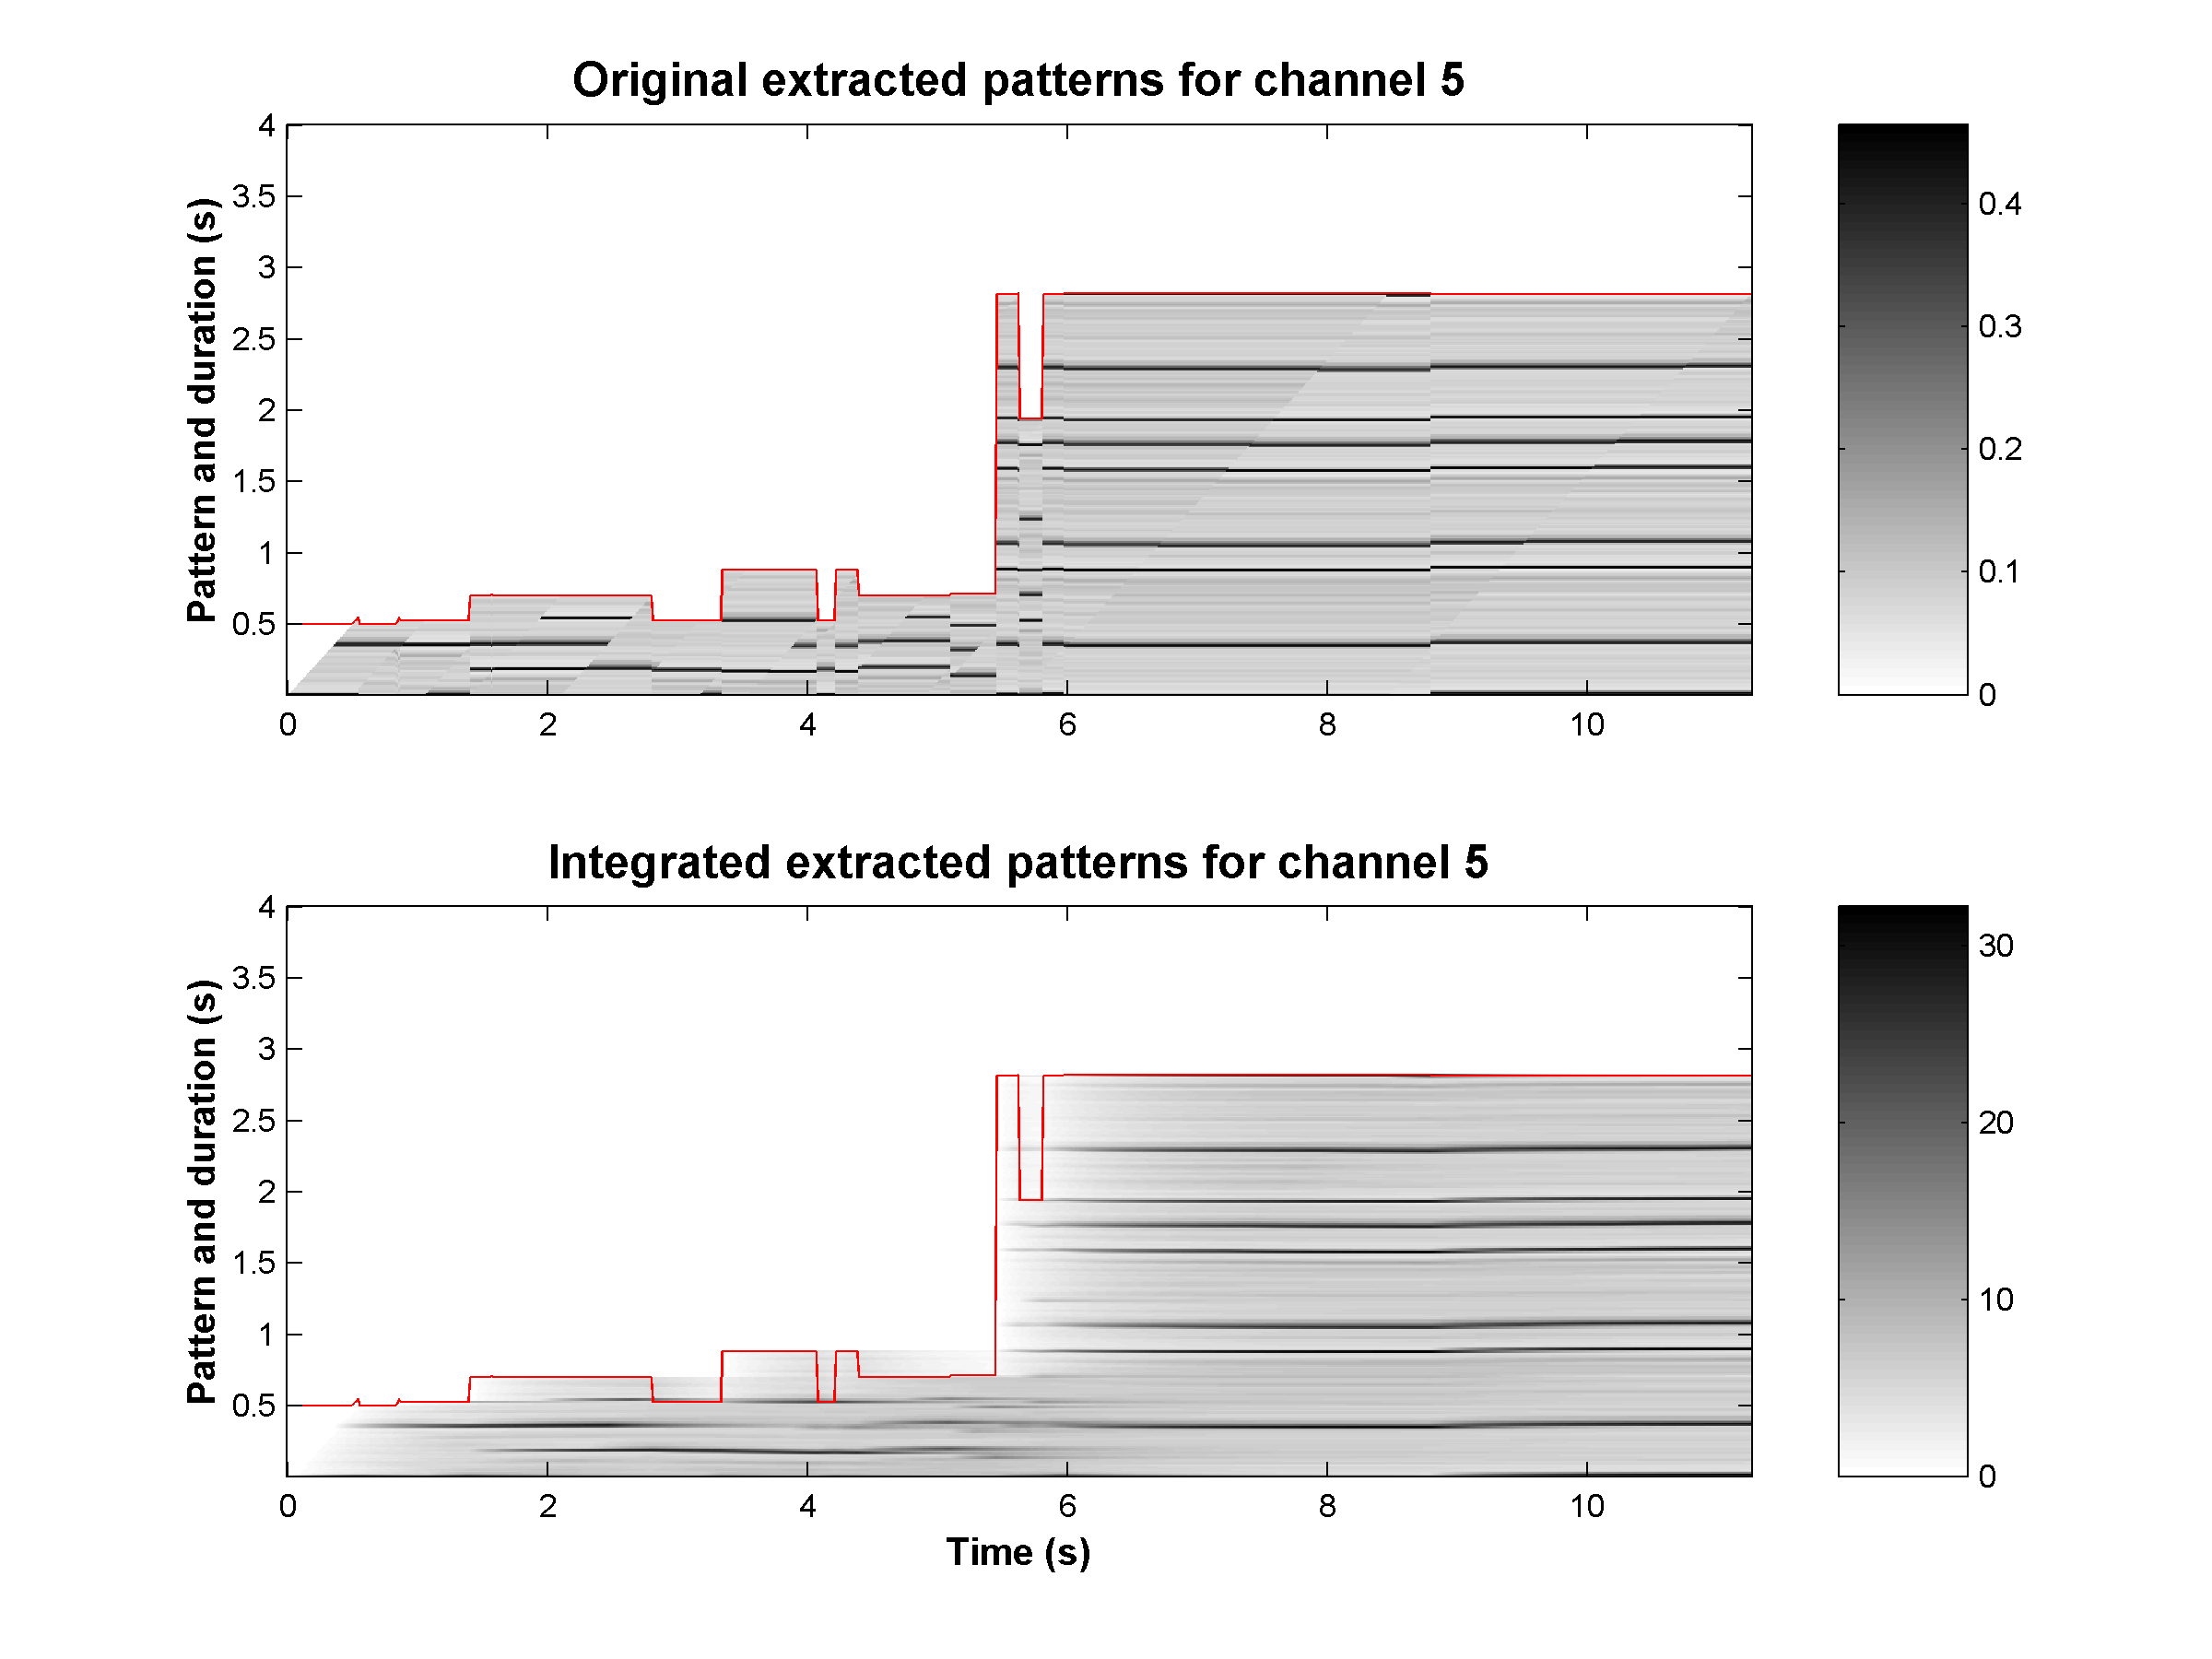
\includegraphics[width=7.5cm]{Graphics/MECDemoPhotekTheLighteningIntegrPattCh5} & 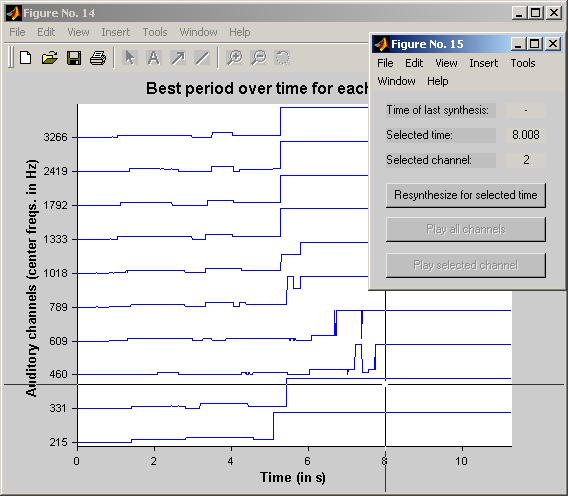
\includegraphics[width=7.5cm]{Graphics/MECDemoPhotekTheLighteningUI}\\
    \end{tabular}
    \caption{Results for PhotekTheLightening.wav}
    \label{Fig:MECPhotekExample}
\end{figure}

% --------------------------------------------------------------------------------
